% Options for packages loaded elsewhere
\PassOptionsToPackage{unicode}{hyperref}
\PassOptionsToPackage{hyphens}{url}
%
\documentclass[
]{article}
\usepackage{amsmath,amssymb}
\usepackage{lmodern}
\usepackage{ifxetex,ifluatex}
\ifnum 0\ifxetex 1\fi\ifluatex 1\fi=0 % if pdftex
  \usepackage[T1]{fontenc}
  \usepackage[utf8]{inputenc}
  \usepackage{textcomp} % provide euro and other symbols
\else % if luatex or xetex
  \usepackage{unicode-math}
  \defaultfontfeatures{Scale=MatchLowercase}
  \defaultfontfeatures[\rmfamily]{Ligatures=TeX,Scale=1}
\fi
% Use upquote if available, for straight quotes in verbatim environments
\IfFileExists{upquote.sty}{\usepackage{upquote}}{}
\IfFileExists{microtype.sty}{% use microtype if available
  \usepackage[]{microtype}
  \UseMicrotypeSet[protrusion]{basicmath} % disable protrusion for tt fonts
}{}
\makeatletter
\@ifundefined{KOMAClassName}{% if non-KOMA class
  \IfFileExists{parskip.sty}{%
    \usepackage{parskip}
  }{% else
    \setlength{\parindent}{0pt}
    \setlength{\parskip}{6pt plus 2pt minus 1pt}}
}{% if KOMA class
  \KOMAoptions{parskip=half}}
\makeatother
\usepackage{xcolor}
\IfFileExists{xurl.sty}{\usepackage{xurl}}{} % add URL line breaks if available
\IfFileExists{bookmark.sty}{\usepackage{bookmark}}{\usepackage{hyperref}}
\hypersetup{
  pdftitle={MovieLens Recommendation System - Code},
  pdfauthor={Uday Adusumilli},
  hidelinks,
  pdfcreator={LaTeX via pandoc}}
\urlstyle{same} % disable monospaced font for URLs
\usepackage[margin=1in]{geometry}
\usepackage{color}
\usepackage{fancyvrb}
\newcommand{\VerbBar}{|}
\newcommand{\VERB}{\Verb[commandchars=\\\{\}]}
\DefineVerbatimEnvironment{Highlighting}{Verbatim}{commandchars=\\\{\}}
% Add ',fontsize=\small' for more characters per line
\newenvironment{Shaded}{}{}
\newcommand{\AlertTok}[1]{\textcolor[rgb]{1.00,0.00,0.00}{\textbf{#1}}}
\newcommand{\AnnotationTok}[1]{\textcolor[rgb]{0.38,0.63,0.69}{\textbf{\textit{#1}}}}
\newcommand{\AttributeTok}[1]{\textcolor[rgb]{0.49,0.56,0.16}{#1}}
\newcommand{\BaseNTok}[1]{\textcolor[rgb]{0.25,0.63,0.44}{#1}}
\newcommand{\BuiltInTok}[1]{#1}
\newcommand{\CharTok}[1]{\textcolor[rgb]{0.25,0.44,0.63}{#1}}
\newcommand{\CommentTok}[1]{\textcolor[rgb]{0.38,0.63,0.69}{\textit{#1}}}
\newcommand{\CommentVarTok}[1]{\textcolor[rgb]{0.38,0.63,0.69}{\textbf{\textit{#1}}}}
\newcommand{\ConstantTok}[1]{\textcolor[rgb]{0.53,0.00,0.00}{#1}}
\newcommand{\ControlFlowTok}[1]{\textcolor[rgb]{0.00,0.44,0.13}{\textbf{#1}}}
\newcommand{\DataTypeTok}[1]{\textcolor[rgb]{0.56,0.13,0.00}{#1}}
\newcommand{\DecValTok}[1]{\textcolor[rgb]{0.25,0.63,0.44}{#1}}
\newcommand{\DocumentationTok}[1]{\textcolor[rgb]{0.73,0.13,0.13}{\textit{#1}}}
\newcommand{\ErrorTok}[1]{\textcolor[rgb]{1.00,0.00,0.00}{\textbf{#1}}}
\newcommand{\ExtensionTok}[1]{#1}
\newcommand{\FloatTok}[1]{\textcolor[rgb]{0.25,0.63,0.44}{#1}}
\newcommand{\FunctionTok}[1]{\textcolor[rgb]{0.02,0.16,0.49}{#1}}
\newcommand{\ImportTok}[1]{#1}
\newcommand{\InformationTok}[1]{\textcolor[rgb]{0.38,0.63,0.69}{\textbf{\textit{#1}}}}
\newcommand{\KeywordTok}[1]{\textcolor[rgb]{0.00,0.44,0.13}{\textbf{#1}}}
\newcommand{\NormalTok}[1]{#1}
\newcommand{\OperatorTok}[1]{\textcolor[rgb]{0.40,0.40,0.40}{#1}}
\newcommand{\OtherTok}[1]{\textcolor[rgb]{0.00,0.44,0.13}{#1}}
\newcommand{\PreprocessorTok}[1]{\textcolor[rgb]{0.74,0.48,0.00}{#1}}
\newcommand{\RegionMarkerTok}[1]{#1}
\newcommand{\SpecialCharTok}[1]{\textcolor[rgb]{0.25,0.44,0.63}{#1}}
\newcommand{\SpecialStringTok}[1]{\textcolor[rgb]{0.73,0.40,0.53}{#1}}
\newcommand{\StringTok}[1]{\textcolor[rgb]{0.25,0.44,0.63}{#1}}
\newcommand{\VariableTok}[1]{\textcolor[rgb]{0.10,0.09,0.49}{#1}}
\newcommand{\VerbatimStringTok}[1]{\textcolor[rgb]{0.25,0.44,0.63}{#1}}
\newcommand{\WarningTok}[1]{\textcolor[rgb]{0.38,0.63,0.69}{\textbf{\textit{#1}}}}
\usepackage{graphicx}
\makeatletter
\def\maxwidth{\ifdim\Gin@nat@width>\linewidth\linewidth\else\Gin@nat@width\fi}
\def\maxheight{\ifdim\Gin@nat@height>\textheight\textheight\else\Gin@nat@height\fi}
\makeatother
% Scale images if necessary, so that they will not overflow the page
% margins by default, and it is still possible to overwrite the defaults
% using explicit options in \includegraphics[width, height, ...]{}
\setkeys{Gin}{width=\maxwidth,height=\maxheight,keepaspectratio}
% Set default figure placement to htbp
\makeatletter
\def\fps@figure{htbp}
\makeatother
\setlength{\emergencystretch}{3em} % prevent overfull lines
\providecommand{\tightlist}{%
  \setlength{\itemsep}{0pt}\setlength{\parskip}{0pt}}
\setcounter{secnumdepth}{5}
\usepackage{booktabs}
\usepackage{longtable}
\usepackage{array}
\usepackage{multirow}
\usepackage{wrapfig}
\usepackage{float}
\usepackage{colortbl}
\usepackage{pdflscape}
\usepackage{tabu}
\usepackage{threeparttable}
\usepackage{threeparttablex}
\usepackage[normalem]{ulem}
\usepackage{makecell}
\usepackage{xcolor}
\ifluatex
  \usepackage{selnolig}  % disable illegal ligatures
\fi

\title{MovieLens Recommendation System - Code}
\author{Uday Adusumilli}
\date{16 Dec, 2021}

\begin{document}
\maketitle

{
\setcounter{tocdepth}{2}
\tableofcontents
}
\begin{Shaded}
\begin{Highlighting}[]
\CommentTok{\# Install all needed libraries if it is not present}

\ControlFlowTok{if}\NormalTok{(}\SpecialCharTok{!}\FunctionTok{require}\NormalTok{(tidyverse)) }\FunctionTok{install.packages}\NormalTok{(}\StringTok{"tidyverse"}\NormalTok{) }
\end{Highlighting}
\end{Shaded}

\begin{verbatim}
## Loading required package: tidyverse
\end{verbatim}

\begin{verbatim}
## -- Attaching packages --------------------------------------- tidyverse 1.3.1 --
\end{verbatim}

\begin{verbatim}
## v ggplot2 3.3.5     v purrr   0.3.4
## v tibble  3.1.2     v dplyr   1.0.7
## v tidyr   1.1.3     v stringr 1.4.0
## v readr   1.4.0     v forcats 0.5.1
\end{verbatim}

\begin{verbatim}
## -- Conflicts ------------------------------------------ tidyverse_conflicts() --
## x dplyr::filter() masks stats::filter()
## x dplyr::lag()    masks stats::lag()
\end{verbatim}

\begin{Shaded}
\begin{Highlighting}[]
\ControlFlowTok{if}\NormalTok{(}\SpecialCharTok{!}\FunctionTok{require}\NormalTok{(kableExtra)) }\FunctionTok{install.packages}\NormalTok{(}\StringTok{"kableExtra"}\NormalTok{)}
\end{Highlighting}
\end{Shaded}

\begin{verbatim}
## Loading required package: kableExtra
\end{verbatim}

\begin{verbatim}
## Warning: package 'kableExtra' was built under R version 4.1.1
\end{verbatim}

\begin{verbatim}
## 
## Attaching package: 'kableExtra'
\end{verbatim}

\begin{verbatim}
## The following object is masked from 'package:dplyr':
## 
##     group_rows
\end{verbatim}

\begin{Shaded}
\begin{Highlighting}[]
\ControlFlowTok{if}\NormalTok{(}\SpecialCharTok{!}\FunctionTok{require}\NormalTok{(tidyr)) }\FunctionTok{install.packages}\NormalTok{(}\StringTok{"tidyr"}\NormalTok{)}
\ControlFlowTok{if}\NormalTok{(}\SpecialCharTok{!}\FunctionTok{require}\NormalTok{(tidyverse)) }\FunctionTok{install.packages}\NormalTok{(}\StringTok{"tidyverse"}\NormalTok{)}
\ControlFlowTok{if}\NormalTok{(}\SpecialCharTok{!}\FunctionTok{require}\NormalTok{(stringr)) }\FunctionTok{install.packages}\NormalTok{(}\StringTok{"stringr"}\NormalTok{)}
\ControlFlowTok{if}\NormalTok{(}\SpecialCharTok{!}\FunctionTok{require}\NormalTok{(forcats)) }\FunctionTok{install.packages}\NormalTok{(}\StringTok{"forcats"}\NormalTok{)}
\ControlFlowTok{if}\NormalTok{(}\SpecialCharTok{!}\FunctionTok{require}\NormalTok{(ggplot2)) }\FunctionTok{install.packages}\NormalTok{(}\StringTok{"ggplot2"}\NormalTok{)}

\ControlFlowTok{if}\NormalTok{(}\SpecialCharTok{!}\FunctionTok{require}\NormalTok{(readr)) }\FunctionTok{install.packages}\NormalTok{(}\StringTok{"readr"}\NormalTok{)}
\ControlFlowTok{if}\NormalTok{(}\SpecialCharTok{!}\FunctionTok{require}\NormalTok{(dplyr)) }\FunctionTok{install.packages}\NormalTok{(}\StringTok{"dplyr"}\NormalTok{)}
\ControlFlowTok{if}\NormalTok{(}\SpecialCharTok{!}\FunctionTok{require}\NormalTok{(gridExtra)) }\FunctionTok{install.packages}\NormalTok{(}\StringTok{"gridExtra"}\NormalTok{)}
\end{Highlighting}
\end{Shaded}

\begin{verbatim}
## Loading required package: gridExtra
\end{verbatim}

\begin{verbatim}
## Warning: package 'gridExtra' was built under R version 4.1.2
\end{verbatim}

\begin{verbatim}
## 
## Attaching package: 'gridExtra'
\end{verbatim}

\begin{verbatim}
## The following object is masked from 'package:dplyr':
## 
##     combine
\end{verbatim}

\begin{Shaded}
\begin{Highlighting}[]
\ControlFlowTok{if}\NormalTok{(}\SpecialCharTok{!}\FunctionTok{require}\NormalTok{(dslabs)) }\FunctionTok{install.packages}\NormalTok{(}\StringTok{"dslabs"}\NormalTok{)}
\end{Highlighting}
\end{Shaded}

\begin{verbatim}
## Loading required package: dslabs
\end{verbatim}

\begin{Shaded}
\begin{Highlighting}[]
\ControlFlowTok{if}\NormalTok{(}\SpecialCharTok{!}\FunctionTok{require}\NormalTok{(data.table)) }\FunctionTok{install.packages}\NormalTok{(}\StringTok{"data.table"}\NormalTok{)}
\end{Highlighting}
\end{Shaded}

\begin{verbatim}
## Loading required package: data.table
\end{verbatim}

\begin{verbatim}
## 
## Attaching package: 'data.table'
\end{verbatim}

\begin{verbatim}
## The following objects are masked from 'package:dplyr':
## 
##     between, first, last
\end{verbatim}

\begin{verbatim}
## The following object is masked from 'package:purrr':
## 
##     transpose
\end{verbatim}

\begin{Shaded}
\begin{Highlighting}[]
\ControlFlowTok{if}\NormalTok{(}\SpecialCharTok{!}\FunctionTok{require}\NormalTok{(ggrepel)) }\FunctionTok{install.packages}\NormalTok{(}\StringTok{"ggrepel"}\NormalTok{)}
\end{Highlighting}
\end{Shaded}

\begin{verbatim}
## Loading required package: ggrepel
\end{verbatim}

\begin{verbatim}
## Warning: package 'ggrepel' was built under R version 4.1.2
\end{verbatim}

\begin{Shaded}
\begin{Highlighting}[]
\ControlFlowTok{if}\NormalTok{(}\SpecialCharTok{!}\FunctionTok{require}\NormalTok{(ggthemes)) }\FunctionTok{install.packages}\NormalTok{(}\StringTok{"ggthemes"}\NormalTok{)}
\end{Highlighting}
\end{Shaded}

\begin{verbatim}
## Loading required package: ggthemes
\end{verbatim}

\begin{verbatim}
## Warning: package 'ggthemes' was built under R version 4.1.2
\end{verbatim}

\begin{Shaded}
\begin{Highlighting}[]
\CommentTok{\# Loading all needed libraries}

\FunctionTok{library}\NormalTok{(dplyr)}
\FunctionTok{library}\NormalTok{(tidyverse)}
\FunctionTok{library}\NormalTok{(kableExtra)}
\FunctionTok{library}\NormalTok{(tidyr)}
\FunctionTok{library}\NormalTok{(stringr)}
\FunctionTok{library}\NormalTok{(forcats)}
\FunctionTok{library}\NormalTok{(ggplot2)}

\FunctionTok{library}\NormalTok{(readr)}
\FunctionTok{library}\NormalTok{(gridExtra)}
\FunctionTok{library}\NormalTok{(dslabs)}
\FunctionTok{library}\NormalTok{(data.table)}
\FunctionTok{library}\NormalTok{(ggrepel)}
\FunctionTok{library}\NormalTok{(ggthemes)}

\DocumentationTok{\#\#\#\#\#\#\#\#\#\#\#\#\#\#\#\#\#\#\#\#\#\#\#\#\#\#\#\#\#\#\#\#\#\#\#\#\#\#\#\#\#\#\#\#\#\#\#\#\#\#\#\#\#\#\#\#\#\#\#\#\#}
\CommentTok{\# Create edx set, validation set, and submission file}
\DocumentationTok{\#\#\#\#\#\#\#\#\#\#\#\#\#\#\#\#\#\#\#\#\#\#\#\#\#\#\#\#\#\#\#\#\#\#\#\#\#\#\#\#\#\#\#\#\#\#\#\#\#\#\#\#\#\#\#\#\#\#\#\#\#}

\CommentTok{\# Note: this process could take a couple of minutes}

\ControlFlowTok{if}\NormalTok{(}\SpecialCharTok{!}\FunctionTok{require}\NormalTok{(tidyverse)) }\FunctionTok{install.packages}\NormalTok{(}\StringTok{"tidyverse"}\NormalTok{, }\AttributeTok{repos =} \StringTok{"http://cran.us.r{-}project.org"}\NormalTok{)}
\ControlFlowTok{if}\NormalTok{(}\SpecialCharTok{!}\FunctionTok{require}\NormalTok{(caret)) }\FunctionTok{install.packages}\NormalTok{(}\StringTok{"caret"}\NormalTok{, }\AttributeTok{repos =} \StringTok{"http://cran.us.r{-}project.org"}\NormalTok{)}
\end{Highlighting}
\end{Shaded}

\begin{verbatim}
## Loading required package: caret
\end{verbatim}

\begin{verbatim}
## Warning: package 'caret' was built under R version 4.1.1
\end{verbatim}

\begin{verbatim}
## Loading required package: lattice
\end{verbatim}

\begin{verbatim}
## 
## Attaching package: 'caret'
\end{verbatim}

\begin{verbatim}
## The following object is masked from 'package:purrr':
## 
##     lift
\end{verbatim}

\begin{Shaded}
\begin{Highlighting}[]
\CommentTok{\# MovieLens 10M dataset:}
\CommentTok{\# https://grouplens.org/datasets/movielens/10m/}
\CommentTok{\# http://files.grouplens.org/datasets/movielens/ml{-}10m.zip}
\end{Highlighting}
\end{Shaded}

The following block needs to be executed if the data isn't available
locally. Execution of the following block requires an active internet
connection.

\begin{Shaded}
\begin{Highlighting}[]
\NormalTok{dl }\OtherTok{\textless{}{-}} \FunctionTok{tempfile}\NormalTok{()}
\FunctionTok{download.file}\NormalTok{(}\StringTok{"http://files.grouplens.org/datasets/movielens/ml{-}10m.zip"}\NormalTok{, dl)}

\NormalTok{ratings }\OtherTok{\textless{}{-}} \FunctionTok{read.table}\NormalTok{(}\AttributeTok{text =} \FunctionTok{gsub}\NormalTok{(}\StringTok{"::"}\NormalTok{, }\StringTok{"}\SpecialCharTok{\textbackslash{}t}\StringTok{"}\NormalTok{, }\FunctionTok{readLines}\NormalTok{(}\FunctionTok{unzip}\NormalTok{(dl, }\StringTok{"ml{-}10M100K/ratings.dat"}\NormalTok{))),}
                      \AttributeTok{col.names =} \FunctionTok{c}\NormalTok{(}\StringTok{"userId"}\NormalTok{, }\StringTok{"movieId"}\NormalTok{, }\StringTok{"rating"}\NormalTok{, }\StringTok{"timestamp"}\NormalTok{))}


\NormalTok{movies }\OtherTok{\textless{}{-}} \FunctionTok{str\_split\_fixed}\NormalTok{(}\FunctionTok{readLines}\NormalTok{(}\FunctionTok{unzip}\NormalTok{(dl, }\StringTok{"ml{-}10M100K/movies.dat"}\NormalTok{)), }\StringTok{"}\SpecialCharTok{\textbackslash{}\textbackslash{}}\StringTok{::"}\NormalTok{, }\DecValTok{3}\NormalTok{)}
\end{Highlighting}
\end{Shaded}

Execution of the following block requires the data files to be preset in
the ml-10M100K folder. The following block is an alternative to the
above block.

\begin{Shaded}
\begin{Highlighting}[]
\NormalTok{ratings }\OtherTok{\textless{}{-}} \FunctionTok{read.table}\NormalTok{(}\AttributeTok{text =} \FunctionTok{gsub}\NormalTok{(}\StringTok{"::"}\NormalTok{, }\StringTok{"}\SpecialCharTok{\textbackslash{}t}\StringTok{"}\NormalTok{, }\FunctionTok{readLines}\NormalTok{(}\StringTok{"ml{-}10M100K/ratings.dat"}\NormalTok{)),}
                      \AttributeTok{col.names =} \FunctionTok{c}\NormalTok{(}\StringTok{"userId"}\NormalTok{, }\StringTok{"movieId"}\NormalTok{, }\StringTok{"rating"}\NormalTok{, }\StringTok{"timestamp"}\NormalTok{))}

\NormalTok{movies }\OtherTok{\textless{}{-}} \FunctionTok{str\_split\_fixed}\NormalTok{(}\FunctionTok{readLines}\NormalTok{(}\StringTok{"ml{-}10M100K/movies.dat"}\NormalTok{), }\StringTok{"}\SpecialCharTok{\textbackslash{}\textbackslash{}}\StringTok{::"}\NormalTok{, }\DecValTok{3}\NormalTok{)}
\end{Highlighting}
\end{Shaded}

With the execution of the above block, data loading is complete.

\begin{Shaded}
\begin{Highlighting}[]
\FunctionTok{colnames}\NormalTok{(movies) }\OtherTok{\textless{}{-}} \FunctionTok{c}\NormalTok{(}\StringTok{"movieId"}\NormalTok{, }\StringTok{"title"}\NormalTok{, }\StringTok{"genres"}\NormalTok{)}

\NormalTok{movies\_old }\OtherTok{\textless{}{-}} \FunctionTok{as.data.frame}\NormalTok{(movies) }\SpecialCharTok{\%\textgreater{}\%} \FunctionTok{mutate}\NormalTok{(}
                                           \AttributeTok{movieId =} \FunctionTok{as.numeric}\NormalTok{(movieId),}
                                           \AttributeTok{title =} \FunctionTok{as.character}\NormalTok{(title),}
                                           \AttributeTok{genres =} \FunctionTok{as.character}\NormalTok{(genres))}\CommentTok{\# modified}

\NormalTok{movies }\OtherTok{=} \FunctionTok{subset}\NormalTok{(movies\_old, }\AttributeTok{select =} \FunctionTok{c}\NormalTok{(movieId,title,genres))}

\NormalTok{movielens }\OtherTok{\textless{}{-}} \FunctionTok{left\_join}\NormalTok{(ratings, movies, }\AttributeTok{by =} \StringTok{"movieId"}\NormalTok{)}

\CommentTok{\# Validation set will be 10\% of MovieLens data}

\FunctionTok{set.seed}\NormalTok{(}\DecValTok{1}\NormalTok{, }\AttributeTok{sample.kind =} \StringTok{"Rounding"}\NormalTok{) }\CommentTok{\# if using R 3.5 or earlier, use \textasciigrave{}set.seed(1)\textasciigrave{} instead}
\end{Highlighting}
\end{Shaded}

\begin{verbatim}
## Warning in set.seed(1, sample.kind = "Rounding"): non-uniform 'Rounding' sampler
## used
\end{verbatim}

\begin{Shaded}
\begin{Highlighting}[]
\NormalTok{test\_index }\OtherTok{\textless{}{-}} \FunctionTok{createDataPartition}\NormalTok{(}\AttributeTok{y =}\NormalTok{ movielens}\SpecialCharTok{$}\NormalTok{rating, }\AttributeTok{times =} \DecValTok{1}\NormalTok{, }\AttributeTok{p =} \FloatTok{0.1}\NormalTok{, }\AttributeTok{list =} \ConstantTok{FALSE}\NormalTok{)}
\NormalTok{edx }\OtherTok{\textless{}{-}}\NormalTok{ movielens[}\SpecialCharTok{{-}}\NormalTok{test\_index,]}
\NormalTok{temp }\OtherTok{\textless{}{-}}\NormalTok{ movielens[test\_index,]}

\CommentTok{\# Make sure userId and movieId in validation set are also in edx set}

\NormalTok{validation }\OtherTok{\textless{}{-}}\NormalTok{ temp }\SpecialCharTok{\%\textgreater{}\%} 
  \FunctionTok{semi\_join}\NormalTok{(edx, }\AttributeTok{by =} \StringTok{"movieId"}\NormalTok{) }\SpecialCharTok{\%\textgreater{}\%}
  \FunctionTok{semi\_join}\NormalTok{(edx, }\AttributeTok{by =} \StringTok{"userId"}\NormalTok{)}

\CommentTok{\# Add rows removed from validation set back into edx set}

\NormalTok{removed }\OtherTok{\textless{}{-}} \FunctionTok{anti\_join}\NormalTok{(temp, validation)}
\end{Highlighting}
\end{Shaded}

\begin{verbatim}
## Joining, by = c("userId", "movieId", "rating", "timestamp", "title", "genres")
\end{verbatim}

\begin{Shaded}
\begin{Highlighting}[]
\NormalTok{edx }\OtherTok{\textless{}{-}} \FunctionTok{rbind}\NormalTok{(edx, removed)}

\FunctionTok{rm}\NormalTok{(dl, ratings, movies, test\_index, temp, movielens, removed)}

\FunctionTok{library}\NormalTok{(kableExtra)}
\end{Highlighting}
\end{Shaded}

Top rows of the Edx file.

\begin{Shaded}
\begin{Highlighting}[]
\FunctionTok{head}\NormalTok{(edx)}
\end{Highlighting}
\end{Shaded}

\begin{verbatim}
##   userId movieId rating timestamp                         title
## 1      1     122      5 838985046              Boomerang (1992)
## 2      1     185      5 838983525               Net, The (1995)
## 4      1     292      5 838983421               Outbreak (1995)
## 5      1     316      5 838983392               Stargate (1994)
## 6      1     329      5 838983392 Star Trek: Generations (1994)
## 7      1     355      5 838984474       Flintstones, The (1994)
##                          genres
## 1                Comedy|Romance
## 2         Action|Crime|Thriller
## 4  Action|Drama|Sci-Fi|Thriller
## 5       Action|Adventure|Sci-Fi
## 6 Action|Adventure|Drama|Sci-Fi
## 7       Children|Comedy|Fantasy
\end{verbatim}

\newpage

\hypertarget{executive-summary}{%
\section{Executive Summary}\label{executive-summary}}

The purpose for this project is creating a recommender system using
MovieLens dataset.

The version of movielens dataset used for this final assignment contains
approximately 10 Milions of movies ratings, divided in 9 Milions for
training and one Milion for validation. It is a small subset of a much
larger (and famous) dataset with several millions of ratings. Into the
training dataset there are approximately \textbf{70.000 users} and
\textbf{11.000 different movies} divided in 20 genres such as Action,
Adventure, Horror, Drama, Thriller and more.

After a initial data exploration, the recommender systems builted on
this dataset are evaluated and choosen based on the RMSE - Root Mean
Squared Error that should be at least lower than \textbf{0.87750}.

\[\mbox{RMSE} = \sqrt{\frac{1}{n}\sum_{t=1}^{n}e_t^2}\]

\begin{Shaded}
\begin{Highlighting}[]
\CommentTok{\# The RMSE function that will be used in this project is:}
\NormalTok{RMSE }\OtherTok{\textless{}{-}} \ControlFlowTok{function}\NormalTok{(}\AttributeTok{true\_ratings =} \ConstantTok{NULL}\NormalTok{, }\AttributeTok{predicted\_ratings =} \ConstantTok{NULL}\NormalTok{) \{}
    \FunctionTok{sqrt}\NormalTok{(}\FunctionTok{mean}\NormalTok{((true\_ratings }\SpecialCharTok{{-}}\NormalTok{ predicted\_ratings)}\SpecialCharTok{\^{}}\DecValTok{2}\NormalTok{))}
\NormalTok{\}}
\end{Highlighting}
\end{Shaded}

For accomplishing this goal, the \textbf{Regularized Movie+User+Genre
Model} is capable to reach a RMSE of \textbf{0.8628}, that is really
good.

\hypertarget{exploratory-data-analysis}{%
\section{Exploratory Data Analysis}\label{exploratory-data-analysis}}

\hypertarget{inital-data-exploration}{%
\subsection{Inital data Exploration}\label{inital-data-exploration}}

The 10 Millions dataset is divided into two dataset: \texttt{edx} for
training purpose and \texttt{validation} for the validation phase.

The \texttt{edx} dataset contains approximately 9 Millions of rows with
70.000 different users and 11.000 movies with rating score between 0.5
and 5. There is no missing values (0 or NA).

\textbf{edx dataset}

\begin{Shaded}
\begin{Highlighting}[]
\NormalTok{edx }\SpecialCharTok{\%\textgreater{}\%} \FunctionTok{summarize}\NormalTok{(}\AttributeTok{Users =} \FunctionTok{n\_distinct}\NormalTok{(userId),}
              \AttributeTok{Movies =} \FunctionTok{n\_distinct}\NormalTok{(movieId)) }\SpecialCharTok{\%\textgreater{}\%} 
\FunctionTok{kable}\NormalTok{() }\SpecialCharTok{\%\textgreater{}\%}
   \FunctionTok{kable\_styling}\NormalTok{(}\AttributeTok{bootstrap\_options =} \FunctionTok{c}\NormalTok{(}\StringTok{"striped"}\NormalTok{, }\StringTok{"hover"}\NormalTok{, }\StringTok{"condensed"}\NormalTok{, }\StringTok{"responsive"}\NormalTok{),}
                 \AttributeTok{position =} \StringTok{"center"}\NormalTok{,}
                 \AttributeTok{font\_size =} \DecValTok{10}\NormalTok{,}
                 \AttributeTok{full\_width =} \ConstantTok{FALSE}\NormalTok{)}
\end{Highlighting}
\end{Shaded}

\begin{table}
\centering\begingroup\fontsize{10}{12}\selectfont

\begin{tabular}{r|r}
\hline
Users & Movies\\
\hline
69878 & 10677\\
\hline
\end{tabular}
\endgroup{}
\end{table}

\textbf{Missing Values per Column}

\begin{Shaded}
\begin{Highlighting}[]
\CommentTok{\# edx \textless{}{-} edx \%\textgreater{}\% select({-}X)}
\CommentTok{\# validation \textless{}{-} validation \%\textgreater{}\% select({-}X)}
\end{Highlighting}
\end{Shaded}

\begin{Shaded}
\begin{Highlighting}[]
\FunctionTok{sapply}\NormalTok{(edx, }\ControlFlowTok{function}\NormalTok{(x) }\FunctionTok{sum}\NormalTok{(}\FunctionTok{is.na}\NormalTok{(x))) }\SpecialCharTok{\%\textgreater{}\%} 
\FunctionTok{kable}\NormalTok{() }\SpecialCharTok{\%\textgreater{}\%}
   \FunctionTok{kable\_styling}\NormalTok{(}\AttributeTok{bootstrap\_options =} \FunctionTok{c}\NormalTok{(}\StringTok{"striped"}\NormalTok{, }\StringTok{"hover"}\NormalTok{, }\StringTok{"condensed"}\NormalTok{, }\StringTok{"responsive"}\NormalTok{),}
                 \AttributeTok{position =} \StringTok{"center"}\NormalTok{,}
                 \AttributeTok{font\_size =} \DecValTok{10}\NormalTok{,}
                 \AttributeTok{full\_width =} \ConstantTok{FALSE}\NormalTok{)}
\end{Highlighting}
\end{Shaded}

\begin{table}
\centering\begingroup\fontsize{10}{12}\selectfont

\begin{tabular}{l|r}
\hline
  & x\\
\hline
userId & 0\\
\hline
movieId & 0\\
\hline
rating & 0\\
\hline
timestamp & 0\\
\hline
title & 0\\
\hline
genres & 0\\
\hline
\end{tabular}
\endgroup{}
\end{table}

The features/variables/columns in both datasets are six:

\begin{itemize}
\tightlist
\item
  \textbf{userId} \texttt{\textless{}integer\textgreater{}} that
  contains the unique identification number for each user.
\item
  \textbf{movieId} \texttt{\textless{}numeric\textgreater{}} that
  contains the unique identification number for each movie.
\item
  \textbf{rating} \texttt{\textless{}numeric\textgreater{}} that
  contains the rating of one movie by one user. Ratings are made on a
  5-Star scale with half-star increments.
\item
  \textbf{timestamp} \texttt{\textless{}integer\textgreater{}} that
  contains the timestamp for one specific rating provided by one user.
\item
  \textbf{title} \texttt{\textless{}character\textgreater{}} that
  contains the title of each movie including the year of the release.
\item
  \textbf{genres} \texttt{\textless{}character\textgreater{}} that
  contains a list of pipe-separated of genre of each movie.
\end{itemize}

\newpage

\textbf{First 6 Rows of edx dataset}

\begin{Shaded}
\begin{Highlighting}[]
\FunctionTok{head}\NormalTok{(edx) }\SpecialCharTok{\%\textgreater{}\%}
   \FunctionTok{kable}\NormalTok{() }\SpecialCharTok{\%\textgreater{}\%}
   \FunctionTok{kable\_styling}\NormalTok{(}\AttributeTok{bootstrap\_options =} \FunctionTok{c}\NormalTok{(}\StringTok{"striped"}\NormalTok{, }\StringTok{"hover"}\NormalTok{, }\StringTok{"condensed"}\NormalTok{, }\StringTok{"responsive"}\NormalTok{),}
                 \AttributeTok{position =} \StringTok{"center"}\NormalTok{,}
                 \AttributeTok{font\_size =} \DecValTok{10}\NormalTok{,}
                 \AttributeTok{full\_width =} \ConstantTok{FALSE}\NormalTok{)}
\end{Highlighting}
\end{Shaded}

\begin{table}
\centering\begingroup\fontsize{10}{12}\selectfont

\begin{tabular}{l|r|r|r|r|l|l}
\hline
  & userId & movieId & rating & timestamp & title & genres\\
\hline
1 & 1 & 122 & 5 & 838985046 & Boomerang (1992) & Comedy|Romance\\
\hline
2 & 1 & 185 & 5 & 838983525 & Net, The (1995) & Action|Crime|Thriller\\
\hline
4 & 1 & 292 & 5 & 838983421 & Outbreak (1995) & Action|Drama|Sci-Fi|Thriller\\
\hline
5 & 1 & 316 & 5 & 838983392 & Stargate (1994) & Action|Adventure|Sci-Fi\\
\hline
6 & 1 & 329 & 5 & 838983392 & Star Trek: Generations (1994) & Action|Adventure|Drama|Sci-Fi\\
\hline
7 & 1 & 355 & 5 & 838984474 & Flintstones, The (1994) & Children|Comedy|Fantasy\\
\hline
\end{tabular}
\endgroup{}
\end{table}

\hypertarget{dataset-pre-processing-and-feature-engineering}{%
\subsection{Dataset Pre-Processing and Feature
Engineering}\label{dataset-pre-processing-and-feature-engineering}}

After a initial data exploration, we notice that the \texttt{genres} are
pipe-separated values. It's necessary to extract them for more
consisten, robust and precise estimate. We also observe that the
\texttt{title} contains the year where the movie war released and this
it could be necessary to predic the movie rating. Finally, we can
extract the year and the month for each rating.

The pre-processing phase is composed by this steps:

\begin{enumerate}
\def\labelenumi{\arabic{enumi}.}
\tightlist
\item
  Convert \texttt{timestamp} to a human readable date format;
\item
  Extract the month and the year from the date;
\item
  Extract the release year for each movie from the title;
\item
  Separate each genre from the pipe-separated value. It increases the
  size of both datasets.
\end{enumerate}

\begin{Shaded}
\begin{Highlighting}[]
\CommentTok{\# Convert timestamp to a human readable date}

\NormalTok{edx}\SpecialCharTok{$}\NormalTok{date }\OtherTok{\textless{}{-}} \FunctionTok{as.POSIXct}\NormalTok{(edx}\SpecialCharTok{$}\NormalTok{timestamp, }\AttributeTok{origin=}\StringTok{"1970{-}01{-}01"}\NormalTok{)}
\NormalTok{validation}\SpecialCharTok{$}\NormalTok{date }\OtherTok{\textless{}{-}} \FunctionTok{as.POSIXct}\NormalTok{(validation}\SpecialCharTok{$}\NormalTok{timestamp, }\AttributeTok{origin=}\StringTok{"1970{-}01{-}01"}\NormalTok{)}
\end{Highlighting}
\end{Shaded}

\begin{Shaded}
\begin{Highlighting}[]
\CommentTok{\# Extract the year and month of rate in both dataset}

\NormalTok{edx}\SpecialCharTok{$}\NormalTok{yearOfRate }\OtherTok{\textless{}{-}} \FunctionTok{format}\NormalTok{(edx}\SpecialCharTok{$}\NormalTok{date,}\StringTok{"\%Y"}\NormalTok{)}
\NormalTok{edx}\SpecialCharTok{$}\NormalTok{monthOfRate }\OtherTok{\textless{}{-}} \FunctionTok{format}\NormalTok{(edx}\SpecialCharTok{$}\NormalTok{date,}\StringTok{"\%m"}\NormalTok{)}

\NormalTok{validation}\SpecialCharTok{$}\NormalTok{yearOfRate }\OtherTok{\textless{}{-}} \FunctionTok{format}\NormalTok{(validation}\SpecialCharTok{$}\NormalTok{date,}\StringTok{"\%Y"}\NormalTok{)}
\NormalTok{validation}\SpecialCharTok{$}\NormalTok{monthOfRate }\OtherTok{\textless{}{-}} \FunctionTok{format}\NormalTok{(validation}\SpecialCharTok{$}\NormalTok{date,}\StringTok{"\%m"}\NormalTok{)}
\end{Highlighting}
\end{Shaded}

\begin{Shaded}
\begin{Highlighting}[]
\CommentTok{\# Extract the year of release for each movie in both dataset}
\CommentTok{\# edx dataset}

\NormalTok{edx }\OtherTok{\textless{}{-}}\NormalTok{ edx }\SpecialCharTok{\%\textgreater{}\%}
   \FunctionTok{mutate}\NormalTok{(}\AttributeTok{title =} \FunctionTok{str\_trim}\NormalTok{(title)) }\SpecialCharTok{\%\textgreater{}\%}
   \FunctionTok{extract}\NormalTok{(title,}
           \FunctionTok{c}\NormalTok{(}\StringTok{"titleTemp"}\NormalTok{, }\StringTok{"release"}\NormalTok{),}
           \AttributeTok{regex =} \StringTok{"\^{}(.*) }\SpecialCharTok{\textbackslash{}\textbackslash{}}\StringTok{(([0{-}9 }\SpecialCharTok{\textbackslash{}\textbackslash{}}\StringTok{{-}]*)}\SpecialCharTok{\textbackslash{}\textbackslash{}}\StringTok{)$"}\NormalTok{,}
           \AttributeTok{remove =}\NormalTok{ F) }\SpecialCharTok{\%\textgreater{}\%}
   \FunctionTok{mutate}\NormalTok{(}\AttributeTok{release =} \FunctionTok{if\_else}\NormalTok{(}\FunctionTok{str\_length}\NormalTok{(release) }\SpecialCharTok{\textgreater{}} \DecValTok{4}\NormalTok{,}
                                \FunctionTok{as.integer}\NormalTok{(}\FunctionTok{str\_split}\NormalTok{(release, }\StringTok{"{-}"}\NormalTok{,}
                                                     \AttributeTok{simplify =}\NormalTok{ T)[}\DecValTok{1}\NormalTok{]),}
                                \FunctionTok{as.integer}\NormalTok{(release))}
\NormalTok{   ) }\SpecialCharTok{\%\textgreater{}\%}
   \FunctionTok{mutate}\NormalTok{(}\AttributeTok{title =} \FunctionTok{if\_else}\NormalTok{(}\FunctionTok{is.na}\NormalTok{(titleTemp),}
\NormalTok{                          title,}
\NormalTok{                          titleTemp)}
\NormalTok{         ) }\SpecialCharTok{\%\textgreater{}\%}
  \FunctionTok{select}\NormalTok{(}\SpecialCharTok{{-}}\NormalTok{titleTemp)}

\CommentTok{\# validation dataset}

\NormalTok{validation }\OtherTok{\textless{}{-}}\NormalTok{ validation }\SpecialCharTok{\%\textgreater{}\%}
   \FunctionTok{mutate}\NormalTok{(}\AttributeTok{title =} \FunctionTok{str\_trim}\NormalTok{(title)) }\SpecialCharTok{\%\textgreater{}\%}
   \FunctionTok{extract}\NormalTok{(title,}
           \FunctionTok{c}\NormalTok{(}\StringTok{"titleTemp"}\NormalTok{, }\StringTok{"release"}\NormalTok{),}
           \AttributeTok{regex =} \StringTok{"\^{}(.*) }\SpecialCharTok{\textbackslash{}\textbackslash{}}\StringTok{(([0{-}9 }\SpecialCharTok{\textbackslash{}\textbackslash{}}\StringTok{{-}]*)}\SpecialCharTok{\textbackslash{}\textbackslash{}}\StringTok{)$"}\NormalTok{,}
           \AttributeTok{remove =}\NormalTok{ F) }\SpecialCharTok{\%\textgreater{}\%}
   \FunctionTok{mutate}\NormalTok{(}\AttributeTok{release =} \FunctionTok{if\_else}\NormalTok{(}\FunctionTok{str\_length}\NormalTok{(release) }\SpecialCharTok{\textgreater{}} \DecValTok{4}\NormalTok{,}
                                \FunctionTok{as.integer}\NormalTok{(}\FunctionTok{str\_split}\NormalTok{(release, }\StringTok{"{-}"}\NormalTok{,}
                                                     \AttributeTok{simplify =}\NormalTok{ T)[}\DecValTok{1}\NormalTok{]),}
                                \FunctionTok{as.integer}\NormalTok{(release))}
\NormalTok{   ) }\SpecialCharTok{\%\textgreater{}\%}
   \FunctionTok{mutate}\NormalTok{(}\AttributeTok{title =} \FunctionTok{if\_else}\NormalTok{(}\FunctionTok{is.na}\NormalTok{(titleTemp),}
\NormalTok{                          title,}
\NormalTok{                          titleTemp)}
\NormalTok{         ) }\SpecialCharTok{\%\textgreater{}\%}
  \FunctionTok{select}\NormalTok{(}\SpecialCharTok{{-}}\NormalTok{titleTemp)}
\end{Highlighting}
\end{Shaded}

\begin{Shaded}
\begin{Highlighting}[]
\CommentTok{\# Extract the genre in edx datasets}

\NormalTok{edx }\OtherTok{\textless{}{-}}\NormalTok{ edx }\SpecialCharTok{\%\textgreater{}\%}
   \FunctionTok{mutate}\NormalTok{(}\AttributeTok{genre =} \FunctionTok{fct\_explicit\_na}\NormalTok{(genres,}
                                       \AttributeTok{na\_level =} \StringTok{"(no genres listed)"}\NormalTok{)}
\NormalTok{          ) }\SpecialCharTok{\%\textgreater{}\%}
   \FunctionTok{separate\_rows}\NormalTok{(genre,}
                 \AttributeTok{sep =} \StringTok{"}\SpecialCharTok{\textbackslash{}\textbackslash{}}\StringTok{|"}\NormalTok{)}
\end{Highlighting}
\end{Shaded}

\begin{Shaded}
\begin{Highlighting}[]
\CommentTok{\# Extract the genre in validation datasets}

\NormalTok{validation }\OtherTok{\textless{}{-}}\NormalTok{ validation }\SpecialCharTok{\%\textgreater{}\%}
   \FunctionTok{mutate}\NormalTok{(}\AttributeTok{genre =} \FunctionTok{fct\_explicit\_na}\NormalTok{(genres,}
                                       \AttributeTok{na\_level =} \StringTok{"(no genres listed)"}\NormalTok{)}
\NormalTok{          ) }\SpecialCharTok{\%\textgreater{}\%}
   \FunctionTok{separate\_rows}\NormalTok{(genre,}
                 \AttributeTok{sep =} \StringTok{"}\SpecialCharTok{\textbackslash{}\textbackslash{}}\StringTok{|"}\NormalTok{)}
\end{Highlighting}
\end{Shaded}

\begin{Shaded}
\begin{Highlighting}[]
\CommentTok{\# remove unnecessary columns on edx and validation dataset}

\NormalTok{edx }\OtherTok{\textless{}{-}}\NormalTok{ edx }\SpecialCharTok{\%\textgreater{}\%} \FunctionTok{select}\NormalTok{(userId, movieId, rating, title, genre, release, yearOfRate, monthOfRate)}

\NormalTok{validation }\OtherTok{\textless{}{-}}\NormalTok{ validation }\SpecialCharTok{\%\textgreater{}\%} \FunctionTok{select}\NormalTok{(userId, movieId, rating, title, genre, release, yearOfRate, monthOfRate)}
\end{Highlighting}
\end{Shaded}

\begin{Shaded}
\begin{Highlighting}[]
\CommentTok{\# Convert the columns into the desidered data type}

\NormalTok{edx}\SpecialCharTok{$}\NormalTok{yearOfRate }\OtherTok{\textless{}{-}} \FunctionTok{as.numeric}\NormalTok{(edx}\SpecialCharTok{$}\NormalTok{yearOfRate)}
\NormalTok{edx}\SpecialCharTok{$}\NormalTok{monthOfRate }\OtherTok{\textless{}{-}} \FunctionTok{as.numeric}\NormalTok{(edx}\SpecialCharTok{$}\NormalTok{monthOfRate)}
\NormalTok{edx}\SpecialCharTok{$}\NormalTok{release }\OtherTok{\textless{}{-}} \FunctionTok{as.numeric}\NormalTok{(edx}\SpecialCharTok{$}\NormalTok{release)}

\NormalTok{validation}\SpecialCharTok{$}\NormalTok{yearOfRate }\OtherTok{\textless{}{-}} \FunctionTok{as.numeric}\NormalTok{(validation}\SpecialCharTok{$}\NormalTok{yearOfRate)}
\NormalTok{validation}\SpecialCharTok{$}\NormalTok{monthOfRate }\OtherTok{\textless{}{-}} \FunctionTok{as.numeric}\NormalTok{(validation}\SpecialCharTok{$}\NormalTok{monthOfRate)}
\NormalTok{validation}\SpecialCharTok{$}\NormalTok{release }\OtherTok{\textless{}{-}} \FunctionTok{as.numeric}\NormalTok{(validation}\SpecialCharTok{$}\NormalTok{release)}
\end{Highlighting}
\end{Shaded}

After preprocessing the data, \texttt{edx} dataset looks like this:

\textbf{Processed edx datadaset}

\begin{Shaded}
\begin{Highlighting}[]
\CommentTok{\# Output the processed dataset}

\FunctionTok{head}\NormalTok{(edx) }\SpecialCharTok{\%\textgreater{}\%}
   \FunctionTok{kable}\NormalTok{() }\SpecialCharTok{\%\textgreater{}\%}
   \FunctionTok{kable\_styling}\NormalTok{(}\AttributeTok{bootstrap\_options =} \FunctionTok{c}\NormalTok{(}\StringTok{"striped"}\NormalTok{, }\StringTok{"hover"}\NormalTok{, }\StringTok{"condensed"}\NormalTok{, }\StringTok{"responsive"}\NormalTok{),}
                 \AttributeTok{position =} \StringTok{"center"}\NormalTok{,}
                 \AttributeTok{font\_size =} \DecValTok{10}\NormalTok{,}
                 \AttributeTok{full\_width =} \ConstantTok{FALSE}\NormalTok{)}
\end{Highlighting}
\end{Shaded}

\begin{table}
\centering\begingroup\fontsize{10}{12}\selectfont

\begin{tabular}{r|r|r|l|l|r|r|r}
\hline
userId & movieId & rating & title & genre & release & yearOfRate & monthOfRate\\
\hline
1 & 122 & 5 & Boomerang & Comedy & 1992 & 1996 & 8\\
\hline
1 & 122 & 5 & Boomerang & Romance & 1992 & 1996 & 8\\
\hline
1 & 185 & 5 & Net, The & Action & 1995 & 1996 & 8\\
\hline
1 & 185 & 5 & Net, The & Crime & 1995 & 1996 & 8\\
\hline
1 & 185 & 5 & Net, The & Thriller & 1995 & 1996 & 8\\
\hline
1 & 292 & 5 & Outbreak & Action & 1995 & 1996 & 8\\
\hline
\end{tabular}
\endgroup{}
\end{table}

\newpage

\hypertarget{rating-distribution}{%
\subsection{Rating Distribution}\label{rating-distribution}}

\textbf{Overview of Rating Distribution}

According to the histogram below, it shows that there are a small amount
of negative votes (below 3). Maybe, the user tends to give a vote if he
liked the movie. Half-Star votes are less common than ``Full-Star''
votes.

\begin{Shaded}
\begin{Highlighting}[]
\FunctionTok{hist}\NormalTok{(edx}\SpecialCharTok{$}\NormalTok{rating, }\AttributeTok{main=}\StringTok{"Distribution of User\textquotesingle{}s Ratings"}\NormalTok{, }\AttributeTok{xlab=}\StringTok{"Rating"}\NormalTok{)}
\end{Highlighting}
\end{Shaded}

\begin{center}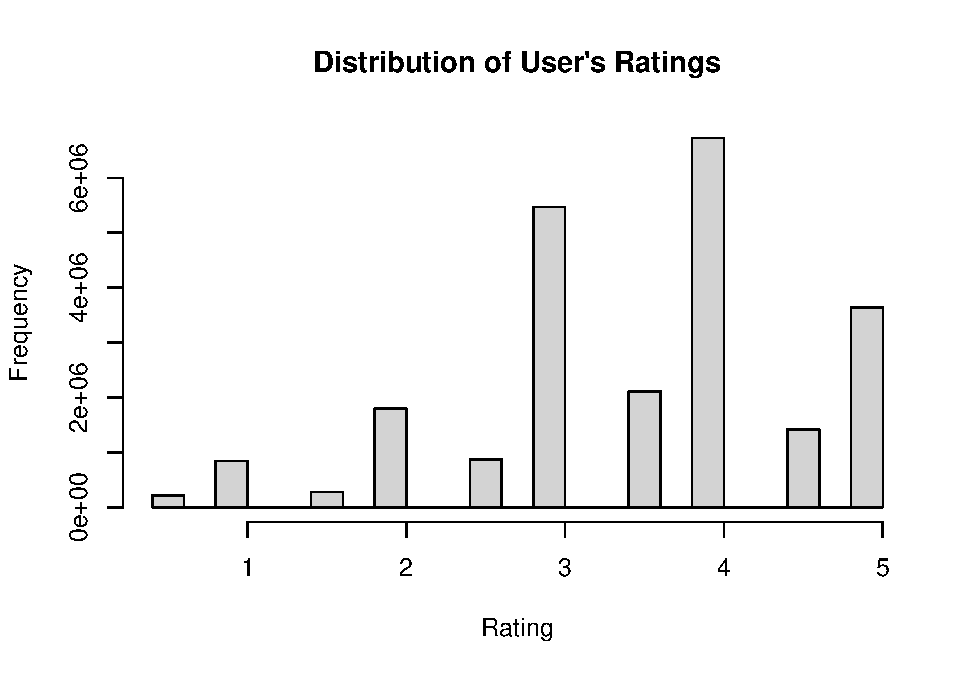
\includegraphics{MovieLens-Project-Code_files/figure-latex/unnamed-chunk-20-1} \end{center}

\textbf{Overview of Rating Frequency through Months and Years}

\begin{Shaded}
\begin{Highlighting}[]
\FunctionTok{hist}\NormalTok{(edx}\SpecialCharTok{$}\NormalTok{monthOfRate, }\AttributeTok{main=}\StringTok{"Frequency of User\textquotesingle{}s Ratings through Month"}\NormalTok{, }\AttributeTok{xlab=}\StringTok{"Month"}\NormalTok{)}
\end{Highlighting}
\end{Shaded}

\begin{center}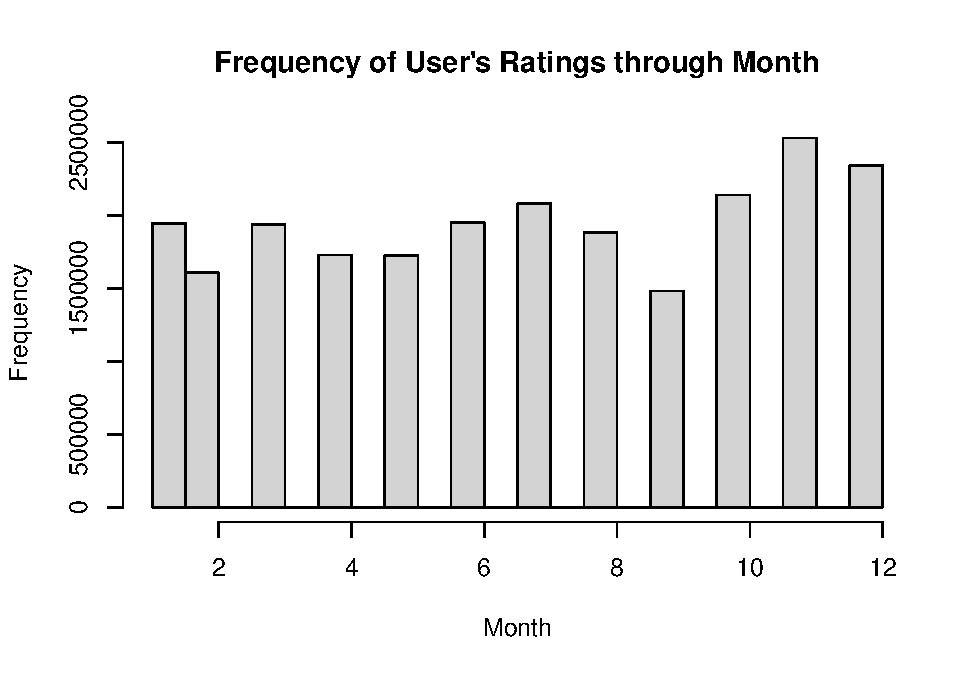
\includegraphics{MovieLens-Project-Code_files/figure-latex/unnamed-chunk-21-1} \end{center}

\begin{Shaded}
\begin{Highlighting}[]
\FunctionTok{hist}\NormalTok{(edx}\SpecialCharTok{$}\NormalTok{yearOfRate, }\AttributeTok{main=}\StringTok{"Frequency of User\textquotesingle{}s Ratings through Years"}\NormalTok{, }\AttributeTok{xlab=}\StringTok{"Years"}\NormalTok{)}
\end{Highlighting}
\end{Shaded}

\begin{center}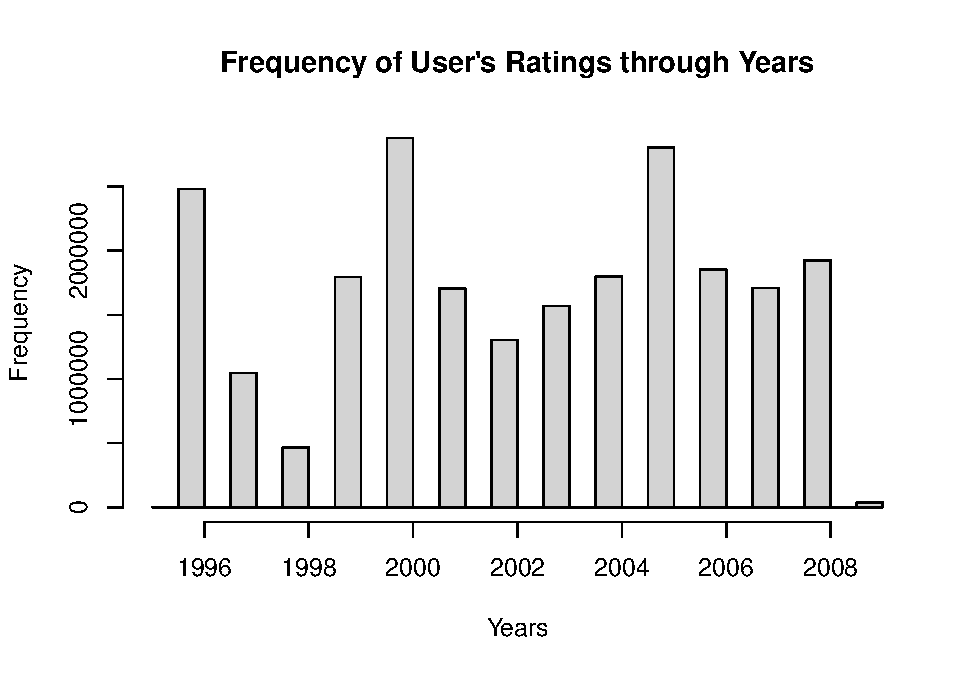
\includegraphics{MovieLens-Project-Code_files/figure-latex/unnamed-chunk-21-2} \end{center}

\hypertarget{numbers-of-ratings-per-movie}{%
\subsubsection{Numbers of Ratings per
Movie}\label{numbers-of-ratings-per-movie}}

\begin{Shaded}
\begin{Highlighting}[]
   \FunctionTok{ggplot}\NormalTok{(edx, }\FunctionTok{aes}\NormalTok{(movieId)) }\SpecialCharTok{+}
   \FunctionTok{theme\_classic}\NormalTok{()  }\SpecialCharTok{+}
   \FunctionTok{geom\_histogram}\NormalTok{(}\AttributeTok{bins=}\DecValTok{500}\NormalTok{) }\SpecialCharTok{+}
   \FunctionTok{labs}\NormalTok{(}\AttributeTok{title =} \StringTok{"Ratings Frequency Distribution Per Title (MovieID)"}\NormalTok{,}
        \AttributeTok{x =} \StringTok{"Title (MovieID)"}\NormalTok{,}
        \AttributeTok{y =} \StringTok{"Frequency"}\NormalTok{)}
\end{Highlighting}
\end{Shaded}

\begin{center}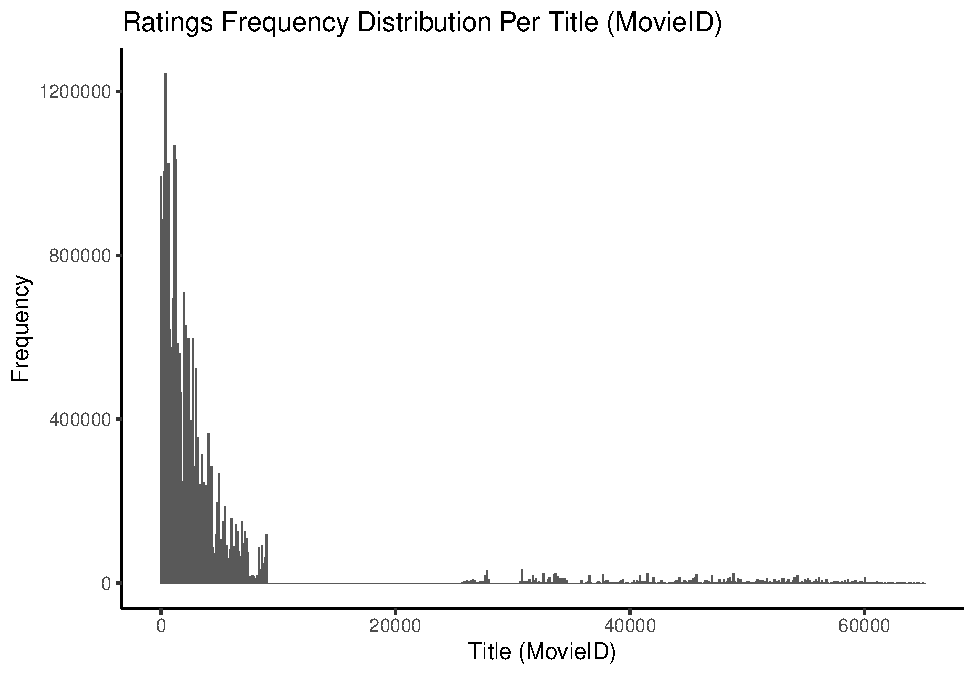
\includegraphics{MovieLens-Project-Code_files/figure-latex/unnamed-chunk-22-1} \end{center}

\hypertarget{top-rated-movies}{%
\subsubsection{Top Rated Movies}\label{top-rated-movies}}

\begin{Shaded}
\begin{Highlighting}[]
\NormalTok{edx }\SpecialCharTok{\%\textgreater{}\%}
   \FunctionTok{group\_by}\NormalTok{(title) }\SpecialCharTok{\%\textgreater{}\%}
   \FunctionTok{summarise}\NormalTok{(}\AttributeTok{count =} \FunctionTok{n}\NormalTok{()) }\SpecialCharTok{\%\textgreater{}\%}
   \FunctionTok{arrange}\NormalTok{(}\FunctionTok{desc}\NormalTok{(count)) }\SpecialCharTok{\%\textgreater{}\%}
   \FunctionTok{head}\NormalTok{(}\AttributeTok{n=}\DecValTok{25}\NormalTok{) }\SpecialCharTok{\%\textgreater{}\%}
   \FunctionTok{ggplot}\NormalTok{(}\FunctionTok{aes}\NormalTok{(title, count)) }\SpecialCharTok{+}
   \FunctionTok{theme\_classic}\NormalTok{()  }\SpecialCharTok{+}
   \FunctionTok{geom\_col}\NormalTok{() }\SpecialCharTok{+}
   \FunctionTok{theme}\NormalTok{(}\AttributeTok{axis.text.x =} \FunctionTok{element\_text}\NormalTok{(}\AttributeTok{angle =} \DecValTok{90}\NormalTok{, }\AttributeTok{hjust =} \DecValTok{1}\NormalTok{, }\AttributeTok{size =} \DecValTok{7}\NormalTok{)) }\SpecialCharTok{+}
   \FunctionTok{labs}\NormalTok{(}\AttributeTok{title =} \StringTok{"Ratings Frequency Distribution Per Title {-} TOP 25 Movies"}\NormalTok{,}
        \AttributeTok{x =} \StringTok{"Title"}\NormalTok{,}
        \AttributeTok{y =} \StringTok{"Frequency"}\NormalTok{)}
\end{Highlighting}
\end{Shaded}

\begin{center}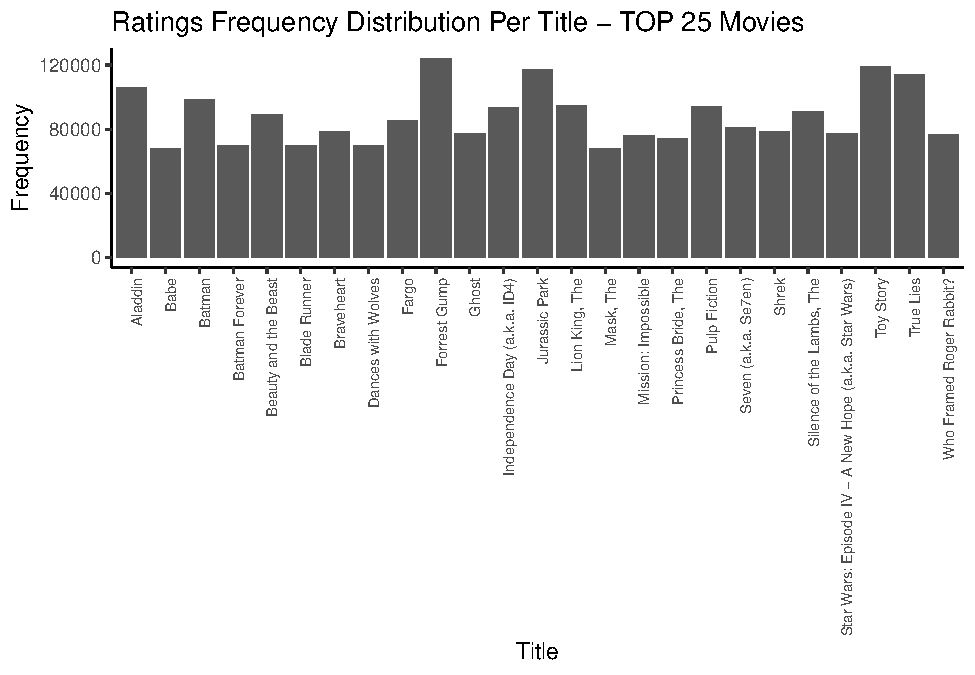
\includegraphics{MovieLens-Project-Code_files/figure-latex/unnamed-chunk-23-1} \end{center}

\begin{Shaded}
\begin{Highlighting}[]
\NormalTok{edx }\SpecialCharTok{\%\textgreater{}\%}
   \FunctionTok{group\_by}\NormalTok{(title) }\SpecialCharTok{\%\textgreater{}\%}
   \FunctionTok{summarise}\NormalTok{(}\AttributeTok{count =} \FunctionTok{n}\NormalTok{()) }\SpecialCharTok{\%\textgreater{}\%}
   \FunctionTok{arrange}\NormalTok{(}\FunctionTok{desc}\NormalTok{(count)) }\SpecialCharTok{\%\textgreater{}\%}
   \FunctionTok{head}\NormalTok{(}\AttributeTok{n=}\DecValTok{25}\NormalTok{) }\SpecialCharTok{\%\textgreater{}\%}
   \FunctionTok{kable}\NormalTok{() }\SpecialCharTok{\%\textgreater{}\%}
   \FunctionTok{kable\_styling}\NormalTok{(}\AttributeTok{bootstrap\_options =} \FunctionTok{c}\NormalTok{(}\StringTok{"striped"}\NormalTok{, }\StringTok{"hover"}\NormalTok{, }\StringTok{"condensed"}\NormalTok{, }\StringTok{"responsive"}\NormalTok{),}
                 \AttributeTok{position =} \StringTok{"center"}\NormalTok{,}
                 \AttributeTok{font\_size =} \DecValTok{10}\NormalTok{,}
                 \AttributeTok{full\_width =} \ConstantTok{FALSE}\NormalTok{)}
\end{Highlighting}
\end{Shaded}

\begin{table}
\centering\begingroup\fontsize{10}{12}\selectfont

\begin{tabular}{l|r}
\hline
title & count\\
\hline
Forrest Gump & 124316\\
\hline
Toy Story & 118950\\
\hline
Jurassic Park & 117440\\
\hline
True Lies & 114115\\
\hline
Aladdin & 105865\\
\hline
Batman & 98340\\
\hline
Lion King, The & 94605\\
\hline
Pulp Fiction & 94086\\
\hline
Independence Day (a.k.a. ID4) & 93796\\
\hline
Silence of the Lambs, The & 91146\\
\hline
Beauty and the Beast & 89145\\
\hline
Fargo & 85580\\
\hline
Seven (a.k.a. Se7en) & 81244\\
\hline
Braveheart & 78636\\
\hline
Shrek & 78378\\
\hline
Ghost & 77440\\
\hline
Star Wars: Episode IV - A New Hope (a.k.a. Star Wars) & 77016\\
\hline
Who Framed Roger Rabbit? & 76825\\
\hline
Mission: Impossible & 75968\\
\hline
Princess Bride, The & 74045\\
\hline
Dances with Wolves & 70101\\
\hline
Blade Runner & 69785\\
\hline
Batman Forever & 69656\\
\hline
Mask, The & 68172\\
\hline
Babe & 68124\\
\hline
\end{tabular}
\endgroup{}
\end{table}

\hypertarget{mean-distribution-per-title-movie-id}{%
\subsubsection{Mean Distribution per Title (Movie
ID)}\label{mean-distribution-per-title-movie-id}}

\begin{Shaded}
\begin{Highlighting}[]
\NormalTok{edx }\SpecialCharTok{\%\textgreater{}\%}
   \FunctionTok{group\_by}\NormalTok{(title) }\SpecialCharTok{\%\textgreater{}\%}
   \FunctionTok{summarise}\NormalTok{(}\AttributeTok{mean =} \FunctionTok{mean}\NormalTok{(rating)) }\SpecialCharTok{\%\textgreater{}\%}
   \FunctionTok{ggplot}\NormalTok{(}\FunctionTok{aes}\NormalTok{(mean)) }\SpecialCharTok{+}
   \FunctionTok{theme\_classic}\NormalTok{()  }\SpecialCharTok{+}
   \FunctionTok{geom\_histogram}\NormalTok{(}\AttributeTok{bins=}\DecValTok{12}\NormalTok{) }\SpecialCharTok{+}
   \FunctionTok{labs}\NormalTok{(}\AttributeTok{title =} \StringTok{"Mean Distribution per Title"}\NormalTok{,}
        \AttributeTok{x =} \StringTok{"Mean"}\NormalTok{,}
        \AttributeTok{y =} \StringTok{"Frequency"}\NormalTok{)}
\end{Highlighting}
\end{Shaded}

\begin{center}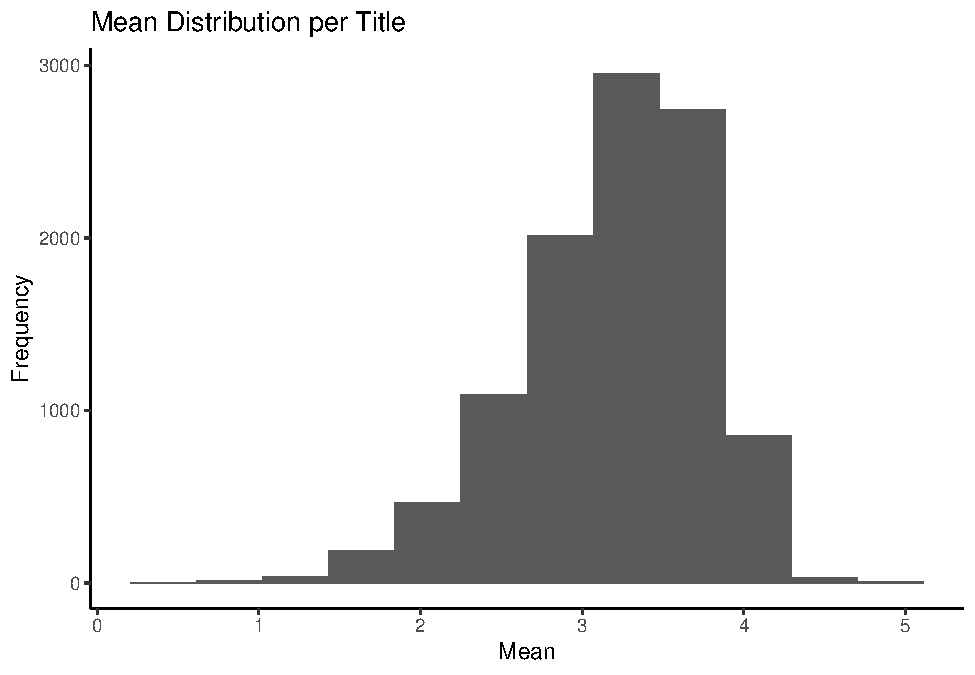
\includegraphics{MovieLens-Project-Code_files/figure-latex/unnamed-chunk-25-1} \end{center}

\begin{Shaded}
\begin{Highlighting}[]
\NormalTok{edx }\SpecialCharTok{\%\textgreater{}\%}
   \FunctionTok{group\_by}\NormalTok{(title) }\SpecialCharTok{\%\textgreater{}\%}
   \FunctionTok{summarise}\NormalTok{(}\AttributeTok{mean =} \FunctionTok{mean}\NormalTok{(rating)) }\SpecialCharTok{\%\textgreater{}\%}
   \FunctionTok{arrange}\NormalTok{(}\FunctionTok{desc}\NormalTok{(mean)) }\SpecialCharTok{\%\textgreater{}\%}
   \FunctionTok{head}\NormalTok{(}\AttributeTok{n=}\DecValTok{25}\NormalTok{) }\SpecialCharTok{\%\textgreater{}\%}
   \FunctionTok{kable}\NormalTok{() }\SpecialCharTok{\%\textgreater{}\%}
   \FunctionTok{kable\_styling}\NormalTok{(}\AttributeTok{bootstrap\_options =} \FunctionTok{c}\NormalTok{(}\StringTok{"striped"}\NormalTok{, }\StringTok{"hover"}\NormalTok{, }\StringTok{"condensed"}\NormalTok{, }\StringTok{"responsive"}\NormalTok{),}
                 \AttributeTok{position =} \StringTok{"center"}\NormalTok{,}
                 \AttributeTok{font\_size =} \DecValTok{10}\NormalTok{,}
                 \AttributeTok{full\_width =} \ConstantTok{FALSE}\NormalTok{)}
\end{Highlighting}
\end{Shaded}

\begin{table}
\centering\begingroup\fontsize{10}{12}\selectfont

\begin{tabular}{l|r}
\hline
title & mean\\
\hline
Blue Light, The (Das Blaue Licht) & 5.000000\\
\hline
Fighting Elegy (Kenka erejii) & 5.000000\\
\hline
Hellhounds on My Trail & 5.000000\\
\hline
Satan's Tango (Sátántangó) & 5.000000\\
\hline
Shadows of Forgotten Ancestors & 5.000000\\
\hline
Sun Alley (Sonnenallee) & 5.000000\\
\hline
Constantine's Sword & 4.750000\\
\hline
Human Condition II, The (Ningen no joken II) & 4.750000\\
\hline
Human Condition III, The (Ningen no joken III) & 4.750000\\
\hline
Who's Singin' Over There? (a.k.a. Who Sings Over There) (Ko to tamo peva) & 4.750000\\
\hline
Class, The (Entre les Murs) & 4.666667\\
\hline
I'm Starting From Three (Ricomincio da Tre) & 4.666667\\
\hline
Bad Blood (Mauvais sang) & 4.500000\\
\hline
Demon Lover Diary & 4.500000\\
\hline
End of Summer, The (Kohayagawa-ke no aki) & 4.500000\\
\hline
Kansas City Confidential & 4.500000\\
\hline
Ladrones & 4.500000\\
\hline
Life of Oharu, The (Saikaku ichidai onna) & 4.500000\\
\hline
Man Named Pearl, A & 4.500000\\
\hline
Mickey & 4.500000\\
\hline
Please Vote for Me & 4.500000\\
\hline
Power of Nightmares: The Rise of the Politics of Fear, The & 4.500000\\
\hline
Testament of Orpheus, The (Testament d'Orphée) & 4.500000\\
\hline
Tokyo! & 4.500000\\
\hline
Valerie and Her Week of Wonders (Valerie a týden divu) & 4.500000\\
\hline
\end{tabular}
\endgroup{}
\end{table}

\hypertarget{median-distribution-per-title-movie-id}{%
\subsubsection{Median Distribution per Title (Movie
ID)}\label{median-distribution-per-title-movie-id}}

\begin{Shaded}
\begin{Highlighting}[]
\NormalTok{edx }\SpecialCharTok{\%\textgreater{}\%}
   \FunctionTok{group\_by}\NormalTok{(title) }\SpecialCharTok{\%\textgreater{}\%}
   \FunctionTok{summarise}\NormalTok{(}\AttributeTok{median =} \FunctionTok{median}\NormalTok{(rating)) }\SpecialCharTok{\%\textgreater{}\%}
   \FunctionTok{ggplot}\NormalTok{(}\FunctionTok{aes}\NormalTok{(median)) }\SpecialCharTok{+}
   \FunctionTok{theme\_classic}\NormalTok{()  }\SpecialCharTok{+}
   \FunctionTok{geom\_histogram}\NormalTok{(}\AttributeTok{bins=}\DecValTok{12}\NormalTok{) }\SpecialCharTok{+}
   \FunctionTok{labs}\NormalTok{(}\AttributeTok{title =} \StringTok{"Median Distribution per Title"}\NormalTok{,}
        \AttributeTok{x =} \StringTok{"Median"}\NormalTok{,}
        \AttributeTok{y =} \StringTok{"Frequency"}\NormalTok{)}
\end{Highlighting}
\end{Shaded}

\begin{center}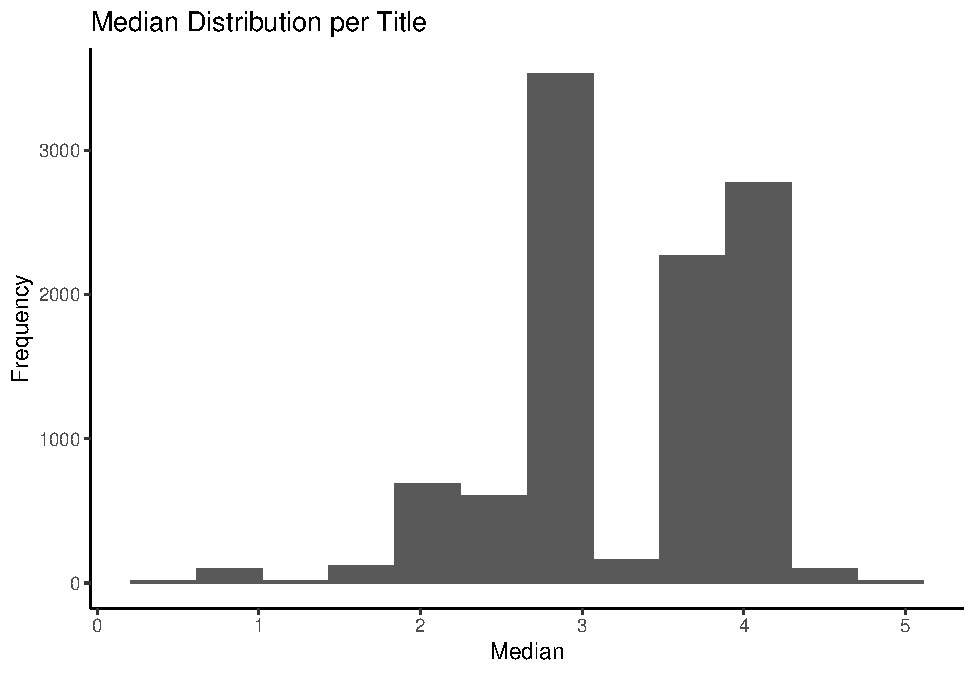
\includegraphics{MovieLens-Project-Code_files/figure-latex/unnamed-chunk-27-1} \end{center}

\begin{Shaded}
\begin{Highlighting}[]
\NormalTok{edx }\SpecialCharTok{\%\textgreater{}\%}
   \FunctionTok{group\_by}\NormalTok{(title) }\SpecialCharTok{\%\textgreater{}\%}
   \FunctionTok{summarise}\NormalTok{(}\AttributeTok{median =} \FunctionTok{median}\NormalTok{(rating)) }\SpecialCharTok{\%\textgreater{}\%}
   \FunctionTok{arrange}\NormalTok{(}\FunctionTok{desc}\NormalTok{(median)) }\SpecialCharTok{\%\textgreater{}\%}
   \FunctionTok{head}\NormalTok{(}\AttributeTok{n=}\DecValTok{25}\NormalTok{) }\SpecialCharTok{\%\textgreater{}\%}
   \FunctionTok{kable}\NormalTok{() }\SpecialCharTok{\%\textgreater{}\%}
   \FunctionTok{kable\_styling}\NormalTok{(}\AttributeTok{bootstrap\_options =} \FunctionTok{c}\NormalTok{(}\StringTok{"striped"}\NormalTok{, }\StringTok{"hover"}\NormalTok{, }\StringTok{"condensed"}\NormalTok{, }\StringTok{"responsive"}\NormalTok{),}
                 \AttributeTok{position =} \StringTok{"center"}\NormalTok{,}
                 \AttributeTok{font\_size =} \DecValTok{10}\NormalTok{,}
                 \AttributeTok{full\_width =} \ConstantTok{FALSE}\NormalTok{)}
\end{Highlighting}
\end{Shaded}

\begin{table}
\centering\begingroup\fontsize{10}{12}\selectfont

\begin{tabular}{l|r}
\hline
title & median\\
\hline
Blue Light, The (Das Blaue Licht) & 5.00\\
\hline
Class, The (Entre les Murs) & 5.00\\
\hline
Fighting Elegy (Kenka erejii) & 5.00\\
\hline
Godfather, The & 5.00\\
\hline
Hellhounds on My Trail & 5.00\\
\hline
Kids of Survival & 5.00\\
\hline
Satan's Tango (Sátántangó) & 5.00\\
\hline
Shadows of Forgotten Ancestors & 5.00\\
\hline
Shawshank Redemption, The & 5.00\\
\hline
Sun Alley (Sonnenallee) & 5.00\\
\hline
Who's Singin' Over There? (a.k.a. Who Sings Over There) (Ko to tamo peva) & 5.00\\
\hline
World of Apu, The (Apur Sansar) & 5.00\\
\hline
Constantine's Sword & 4.75\\
\hline
Human Condition II, The (Ningen no joken II) & 4.75\\
\hline
Human Condition III, The (Ningen no joken III) & 4.75\\
\hline
400 Blows, The (Les Quatre cents coups) & 4.50\\
\hline
49 Up & 4.50\\
\hline
Amelie (Fabuleux destin d'Amélie Poulain, Le) & 4.50\\
\hline
American Beauty & 4.50\\
\hline
Andrei Rublev (Andrey Rublyov) & 4.50\\
\hline
Bad Blood (Mauvais sang) & 4.50\\
\hline
Best of Youth, The (La Meglio gioventù) & 4.50\\
\hline
Cabeza de Vaca & 4.50\\
\hline
Casablanca & 4.50\\
\hline
Celebration, The (Festen) & 4.50\\
\hline
\end{tabular}
\endgroup{}
\end{table}

\hypertarget{genre-analysis}{%
\subsection{Genre Analysis}\label{genre-analysis}}

\hypertarget{rating-distribution-per-genre}{%
\subsubsection{Rating Distribution per
Genre}\label{rating-distribution-per-genre}}

\textbf{Overview of Rating distribution over Genre}

\begin{Shaded}
\begin{Highlighting}[]
\NormalTok{edx }\SpecialCharTok{\%\textgreater{}\%}
   \FunctionTok{group\_by}\NormalTok{(genre) }\SpecialCharTok{\%\textgreater{}\%}
   \FunctionTok{summarise}\NormalTok{(}\AttributeTok{count =} \FunctionTok{n}\NormalTok{()) }\SpecialCharTok{\%\textgreater{}\%}
   \FunctionTok{ggplot}\NormalTok{(}\FunctionTok{aes}\NormalTok{(genre, count)) }\SpecialCharTok{+}
   \FunctionTok{theme\_classic}\NormalTok{()  }\SpecialCharTok{+}
   \FunctionTok{geom\_col}\NormalTok{() }\SpecialCharTok{+}
   \FunctionTok{theme}\NormalTok{(}\AttributeTok{axis.text.x =} \FunctionTok{element\_text}\NormalTok{(}\AttributeTok{angle =} \DecValTok{90}\NormalTok{, }\AttributeTok{hjust =} \DecValTok{1}\NormalTok{)) }\SpecialCharTok{+}
   \FunctionTok{labs}\NormalTok{(}\AttributeTok{title =} \StringTok{"Ratings Frequency Distribution Per Genre"}\NormalTok{,}
        \AttributeTok{x =} \StringTok{"Genre"}\NormalTok{,}
        \AttributeTok{y =} \StringTok{"Frequency"}\NormalTok{)}
\end{Highlighting}
\end{Shaded}

\begin{center}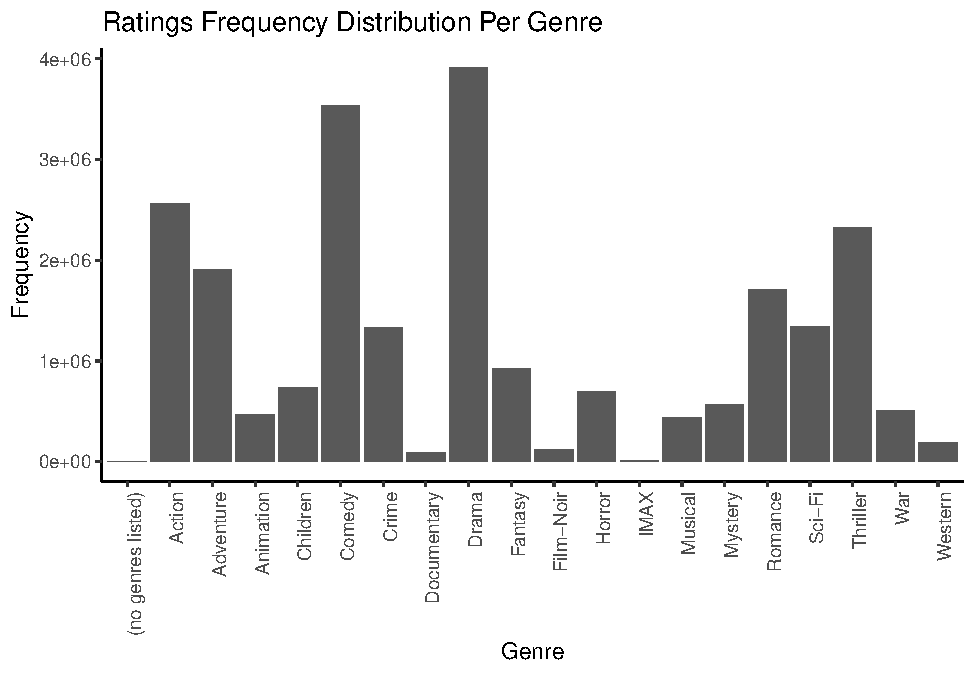
\includegraphics{MovieLens-Project-Code_files/figure-latex/unnamed-chunk-29-1} \end{center}

\begin{Shaded}
\begin{Highlighting}[]
\NormalTok{edx }\SpecialCharTok{\%\textgreater{}\%}
   \FunctionTok{group\_by}\NormalTok{(genre) }\SpecialCharTok{\%\textgreater{}\%}
   \FunctionTok{summarise}\NormalTok{(}\AttributeTok{count =} \FunctionTok{n}\NormalTok{()) }\SpecialCharTok{\%\textgreater{}\%}
   \FunctionTok{arrange}\NormalTok{(}\FunctionTok{desc}\NormalTok{(count)) }\SpecialCharTok{\%\textgreater{}\%}
   \FunctionTok{kable}\NormalTok{() }\SpecialCharTok{\%\textgreater{}\%}
   \FunctionTok{kable\_styling}\NormalTok{(}\AttributeTok{bootstrap\_options =} \FunctionTok{c}\NormalTok{(}\StringTok{"striped"}\NormalTok{, }\StringTok{"hover"}\NormalTok{, }\StringTok{"condensed"}\NormalTok{, }\StringTok{"responsive"}\NormalTok{),}
                 \AttributeTok{position =} \StringTok{"center"}\NormalTok{,}
                 \AttributeTok{font\_size =} \DecValTok{10}\NormalTok{,}
                 \AttributeTok{full\_width =} \ConstantTok{FALSE}\NormalTok{)}
\end{Highlighting}
\end{Shaded}

\begin{table}
\centering\begingroup\fontsize{10}{12}\selectfont

\begin{tabular}{l|r}
\hline
genre & count\\
\hline
Drama & 3910127\\
\hline
Comedy & 3540930\\
\hline
Action & 2560545\\
\hline
Thriller & 2325899\\
\hline
Adventure & 1908892\\
\hline
Romance & 1712100\\
\hline
Sci-Fi & 1341183\\
\hline
Crime & 1327715\\
\hline
Fantasy & 925637\\
\hline
Children & 737994\\
\hline
Horror & 691485\\
\hline
Mystery & 568332\\
\hline
War & 511147\\
\hline
Animation & 467168\\
\hline
Musical & 433080\\
\hline
Western & 189394\\
\hline
Film-Noir & 118541\\
\hline
Documentary & 93066\\
\hline
IMAX & 8181\\
\hline
(no genres listed) & 7\\
\hline
\end{tabular}
\endgroup{}
\end{table}

\hypertarget{mean-distribution-per-genre}{%
\subsubsection{Mean Distribution per
Genre}\label{mean-distribution-per-genre}}

\begin{Shaded}
\begin{Highlighting}[]
\NormalTok{edx }\SpecialCharTok{\%\textgreater{}\%}
   \FunctionTok{group\_by}\NormalTok{(genre) }\SpecialCharTok{\%\textgreater{}\%}
   \FunctionTok{summarise}\NormalTok{(}\AttributeTok{mean =} \FunctionTok{mean}\NormalTok{(rating)) }\SpecialCharTok{\%\textgreater{}\%}
   \FunctionTok{ggplot}\NormalTok{(}\FunctionTok{aes}\NormalTok{(genre, mean)) }\SpecialCharTok{+}
   \FunctionTok{theme\_classic}\NormalTok{()  }\SpecialCharTok{+}
   \FunctionTok{geom\_col}\NormalTok{() }\SpecialCharTok{+}
   \FunctionTok{theme}\NormalTok{(}\AttributeTok{axis.text.x =} \FunctionTok{element\_text}\NormalTok{(}\AttributeTok{angle =} \DecValTok{90}\NormalTok{, }\AttributeTok{hjust =} \DecValTok{1}\NormalTok{)) }\SpecialCharTok{+}
   \FunctionTok{labs}\NormalTok{(}\AttributeTok{title =} \StringTok{"Mean Distribution per Genre"}\NormalTok{,}
        \AttributeTok{x =} \StringTok{"Genre"}\NormalTok{,}
        \AttributeTok{y =} \StringTok{"Mean"}\NormalTok{)}
\end{Highlighting}
\end{Shaded}

\begin{center}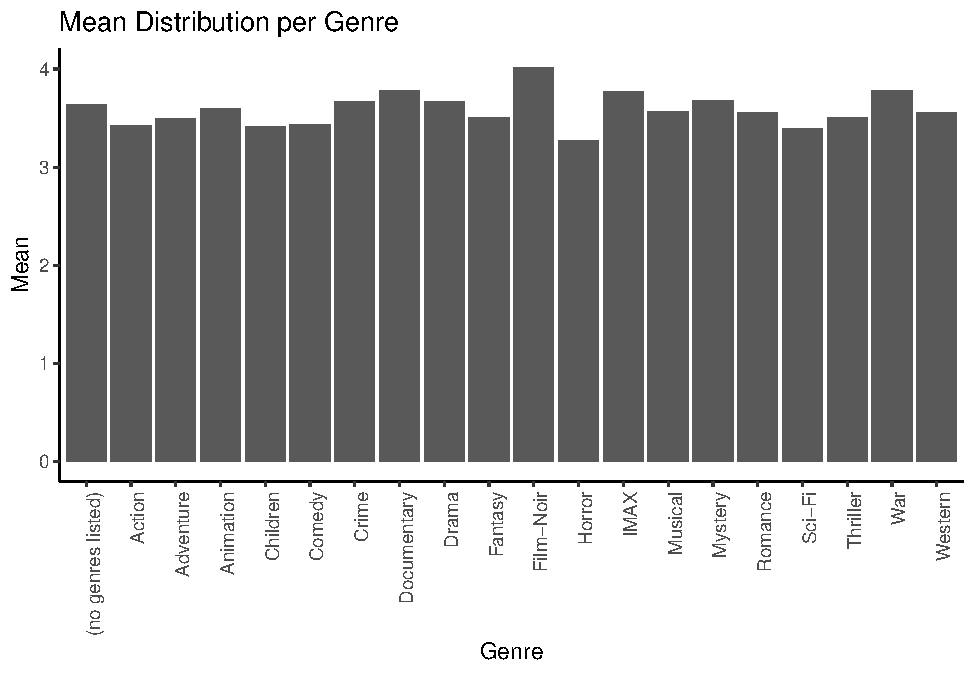
\includegraphics{MovieLens-Project-Code_files/figure-latex/unnamed-chunk-31-1} \end{center}

\begin{Shaded}
\begin{Highlighting}[]
\NormalTok{edx }\SpecialCharTok{\%\textgreater{}\%}
   \FunctionTok{group\_by}\NormalTok{(genre) }\SpecialCharTok{\%\textgreater{}\%}
   \FunctionTok{summarise}\NormalTok{(}\AttributeTok{mean =} \FunctionTok{mean}\NormalTok{(rating)) }\SpecialCharTok{\%\textgreater{}\%}
   \FunctionTok{arrange}\NormalTok{(}\FunctionTok{desc}\NormalTok{(mean)) }\SpecialCharTok{\%\textgreater{}\%}
   \FunctionTok{head}\NormalTok{(}\AttributeTok{n=}\DecValTok{35}\NormalTok{) }\SpecialCharTok{\%\textgreater{}\%}
   \FunctionTok{kable}\NormalTok{() }\SpecialCharTok{\%\textgreater{}\%}
   \FunctionTok{kable\_styling}\NormalTok{(}\AttributeTok{bootstrap\_options =} \FunctionTok{c}\NormalTok{(}\StringTok{"striped"}\NormalTok{, }\StringTok{"hover"}\NormalTok{, }\StringTok{"condensed"}\NormalTok{, }\StringTok{"responsive"}\NormalTok{),}
                 \AttributeTok{position =} \StringTok{"center"}\NormalTok{,}
                 \AttributeTok{font\_size =} \DecValTok{10}\NormalTok{,}
                 \AttributeTok{full\_width =} \ConstantTok{FALSE}\NormalTok{)}
\end{Highlighting}
\end{Shaded}

\begin{table}
\centering\begingroup\fontsize{10}{12}\selectfont

\begin{tabular}{l|r}
\hline
genre & mean\\
\hline
Film-Noir & 4.011625\\
\hline
Documentary & 3.783487\\
\hline
War & 3.780813\\
\hline
IMAX & 3.767693\\
\hline
Mystery & 3.677001\\
\hline
Drama & 3.673131\\
\hline
Crime & 3.665925\\
\hline
(no genres listed) & 3.642857\\
\hline
Animation & 3.600644\\
\hline
Musical & 3.563305\\
\hline
Western & 3.555918\\
\hline
Romance & 3.553813\\
\hline
Thriller & 3.507676\\
\hline
Fantasy & 3.501946\\
\hline
Adventure & 3.493544\\
\hline
Comedy & 3.436908\\
\hline
Action & 3.421405\\
\hline
Children & 3.418715\\
\hline
Sci-Fi & 3.395743\\
\hline
Horror & 3.269815\\
\hline
\end{tabular}
\endgroup{}
\end{table}

\hypertarget{median-distribution-per-genre}{%
\subsubsection{Median Distribution per
Genre}\label{median-distribution-per-genre}}

\begin{Shaded}
\begin{Highlighting}[]
\NormalTok{edx }\SpecialCharTok{\%\textgreater{}\%}
   \FunctionTok{group\_by}\NormalTok{(genre) }\SpecialCharTok{\%\textgreater{}\%}
   \FunctionTok{summarise}\NormalTok{(}\AttributeTok{median =} \FunctionTok{median}\NormalTok{(rating)) }\SpecialCharTok{\%\textgreater{}\%}
   \FunctionTok{ggplot}\NormalTok{(}\FunctionTok{aes}\NormalTok{(genre, median)) }\SpecialCharTok{+}
   \FunctionTok{theme\_classic}\NormalTok{()  }\SpecialCharTok{+}
   \FunctionTok{geom\_col}\NormalTok{() }\SpecialCharTok{+}
   \FunctionTok{theme}\NormalTok{(}\AttributeTok{axis.text.x =} \FunctionTok{element\_text}\NormalTok{(}\AttributeTok{angle =} \DecValTok{90}\NormalTok{, }\AttributeTok{hjust =} \DecValTok{1}\NormalTok{)) }\SpecialCharTok{+}
   \FunctionTok{labs}\NormalTok{(}\AttributeTok{title =} \StringTok{"Median Distribution per Genre"}\NormalTok{,}
        \AttributeTok{x =} \StringTok{"Genre"}\NormalTok{,}
        \AttributeTok{y =} \StringTok{"Median"}\NormalTok{)}
\end{Highlighting}
\end{Shaded}

\begin{center}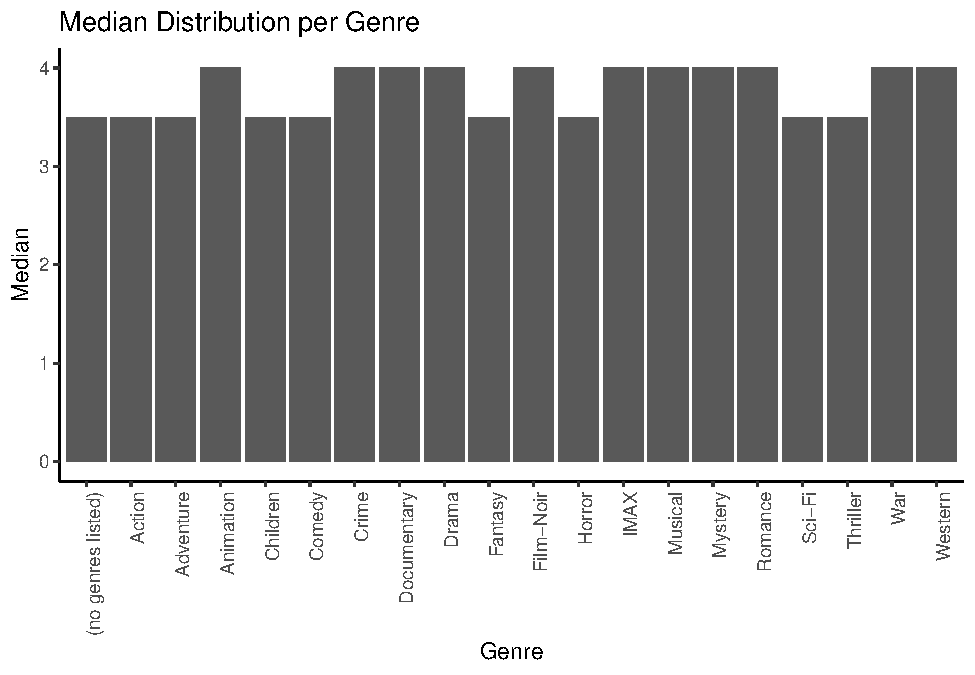
\includegraphics{MovieLens-Project-Code_files/figure-latex/unnamed-chunk-33-1} \end{center}

\begin{Shaded}
\begin{Highlighting}[]
\NormalTok{edx }\SpecialCharTok{\%\textgreater{}\%}
   \FunctionTok{group\_by}\NormalTok{(genre) }\SpecialCharTok{\%\textgreater{}\%}
   \FunctionTok{summarise}\NormalTok{(}\AttributeTok{median =} \FunctionTok{median}\NormalTok{(rating)) }\SpecialCharTok{\%\textgreater{}\%}
   \FunctionTok{arrange}\NormalTok{(}\FunctionTok{desc}\NormalTok{(median)) }\SpecialCharTok{\%\textgreater{}\%}
   \FunctionTok{head}\NormalTok{(}\AttributeTok{n=}\DecValTok{35}\NormalTok{) }\SpecialCharTok{\%\textgreater{}\%}
   \FunctionTok{kable}\NormalTok{() }\SpecialCharTok{\%\textgreater{}\%}
   \FunctionTok{kable\_styling}\NormalTok{(}\AttributeTok{bootstrap\_options =} \FunctionTok{c}\NormalTok{(}\StringTok{"striped"}\NormalTok{, }\StringTok{"hover"}\NormalTok{, }\StringTok{"condensed"}\NormalTok{, }\StringTok{"responsive"}\NormalTok{),}
                 \AttributeTok{position =} \StringTok{"center"}\NormalTok{,}
                 \AttributeTok{font\_size =} \DecValTok{10}\NormalTok{,}
                 \AttributeTok{full\_width =} \ConstantTok{FALSE}\NormalTok{)}
\end{Highlighting}
\end{Shaded}

\begin{table}
\centering\begingroup\fontsize{10}{12}\selectfont

\begin{tabular}{l|r}
\hline
genre & median\\
\hline
Animation & 4.0\\
\hline
Crime & 4.0\\
\hline
Documentary & 4.0\\
\hline
Drama & 4.0\\
\hline
Film-Noir & 4.0\\
\hline
IMAX & 4.0\\
\hline
Musical & 4.0\\
\hline
Mystery & 4.0\\
\hline
Romance & 4.0\\
\hline
War & 4.0\\
\hline
Western & 4.0\\
\hline
(no genres listed) & 3.5\\
\hline
Action & 3.5\\
\hline
Adventure & 3.5\\
\hline
Children & 3.5\\
\hline
Comedy & 3.5\\
\hline
Fantasy & 3.5\\
\hline
Horror & 3.5\\
\hline
Sci-Fi & 3.5\\
\hline
Thriller & 3.5\\
\hline
\end{tabular}
\endgroup{}
\end{table}

\hypertarget{analysis---model-building-and-evaluation}{%
\section{Analysis - Model Building and
Evaluation}\label{analysis---model-building-and-evaluation}}

\hypertarget{naive-baseline-model}{%
\subsection{Naive Baseline Model}\label{naive-baseline-model}}

The simplest model that someone can build, is a Naive Model that predict
ALWAYS the mean. In this case, the mean is approximately 3.5.

\begin{Shaded}
\begin{Highlighting}[]
\FunctionTok{paste}\NormalTok{(}\StringTok{"The mean is:"}\NormalTok{, }\FunctionTok{as.character}\NormalTok{(}\FunctionTok{mean}\NormalTok{(edx}\SpecialCharTok{$}\NormalTok{rating)))}
\end{Highlighting}
\end{Shaded}

\begin{verbatim}
## [1] "The mean is: 3.52701897954609"
\end{verbatim}

\hypertarget{naive-mean-baseline-model}{%
\subsubsection{Naive Mean-Baseline
Model}\label{naive-mean-baseline-model}}

The formula used is:

\[Y_{u,i} = \hat{\mu} + \varepsilon_{u,i}\]

With \(\hat{\mu}\) is the mean and \(\varepsilon_{i,u}\) is the
independent errors sampled from the same distribution centered at 0.

\begin{Shaded}
\begin{Highlighting}[]
\CommentTok{\# Calculate the average of all movies}

\NormalTok{mu\_hat }\OtherTok{\textless{}{-}} \FunctionTok{mean}\NormalTok{(edx}\SpecialCharTok{$}\NormalTok{rating)}

\CommentTok{\# Predict the RMSE on the validation set}

\NormalTok{rmse\_mean\_model\_result }\OtherTok{\textless{}{-}} \FunctionTok{RMSE}\NormalTok{(validation}\SpecialCharTok{$}\NormalTok{rating, mu\_hat)}

\CommentTok{\# Creating a results dataframe that contains all RMSE results}

\NormalTok{results }\OtherTok{\textless{}{-}} \FunctionTok{data.frame}\NormalTok{(}\AttributeTok{model=}\StringTok{"Naive Mean{-}Baseline Model"}\NormalTok{, }\AttributeTok{RMSE=}\NormalTok{rmse\_mean\_model\_result)}
\end{Highlighting}
\end{Shaded}

The RMSE on the \texttt{validation} dataset is \textbf{1.05}. It is very
far for the target RMSE (below 0.87) and that indicates poor performance
for the model.

\hypertarget{movie-based-model-a-content-based-approach}{%
\subsection{Movie-Based Model, a Content-based
Approach}\label{movie-based-model-a-content-based-approach}}

The first Non-Naive Model takes into account the content. In this case
the movies that are rated higher or lower resperct to each other.

The formula used is:

\[Y_{u,i} = \hat{\mu} + b_i + \epsilon_{u,i}\]

With \(\hat{\mu}\) is the mean and \(\varepsilon_{i,u}\) is the
independent errors sampled from the same distribution centered at 0. The
\(b_i\) is a measure for the popularity of movie \(i\), i.e.~the bias of
movie \(i\).

\begin{Shaded}
\begin{Highlighting}[]
\CommentTok{\# Calculate the average of all movies}

\NormalTok{mu\_hat }\OtherTok{\textless{}{-}} \FunctionTok{mean}\NormalTok{(edx}\SpecialCharTok{$}\NormalTok{rating)}

\CommentTok{\# Calculate the average by movie}

\NormalTok{movie\_avgs }\OtherTok{\textless{}{-}}\NormalTok{ edx }\SpecialCharTok{\%\textgreater{}\%}
   \FunctionTok{group\_by}\NormalTok{(movieId) }\SpecialCharTok{\%\textgreater{}\%}
   \FunctionTok{summarize}\NormalTok{(}\AttributeTok{b\_i =} \FunctionTok{mean}\NormalTok{(rating }\SpecialCharTok{{-}}\NormalTok{ mu\_hat))}

\CommentTok{\# Compute the predicted ratings on validation dataset}

\NormalTok{rmse\_movie\_model }\OtherTok{\textless{}{-}}\NormalTok{ validation }\SpecialCharTok{\%\textgreater{}\%}
   \FunctionTok{left\_join}\NormalTok{(movie\_avgs, }\AttributeTok{by=}\StringTok{\textquotesingle{}movieId\textquotesingle{}}\NormalTok{) }\SpecialCharTok{\%\textgreater{}\%}
   \FunctionTok{mutate}\NormalTok{(}\AttributeTok{pred =}\NormalTok{ mu\_hat }\SpecialCharTok{+}\NormalTok{ b\_i) }\SpecialCharTok{\%\textgreater{}\%}
   \FunctionTok{pull}\NormalTok{(pred)}

\NormalTok{rmse\_movie\_model\_result }\OtherTok{\textless{}{-}} \FunctionTok{RMSE}\NormalTok{(validation}\SpecialCharTok{$}\NormalTok{rating, rmse\_movie\_model)}

\CommentTok{\# Adding the results to the results dataset}

\NormalTok{results }\OtherTok{\textless{}{-}}\NormalTok{ results }\SpecialCharTok{\%\textgreater{}\%} \FunctionTok{add\_row}\NormalTok{(}\AttributeTok{model=}\StringTok{"Movie{-}Based Model"}\NormalTok{, }\AttributeTok{RMSE=}\NormalTok{rmse\_movie\_model\_result)}
\end{Highlighting}
\end{Shaded}

The RMSE on the \texttt{validation} dataset is \textbf{0.94}. It better
than the Naive Mean-Baseline Model, but it is also very far from the
target RMSE (below 0.87) and that indicates poor performance for the
model.

\hypertarget{movie-user-model-a-user-based-approach}{%
\subsection{Movie + User Model, a User-based
approach}\label{movie-user-model-a-user-based-approach}}

The second Non-Naive Model consider that the users have different tastes
and rate differently.

The formula used is:

\[Y_{u,i} = \hat{\mu} + b_i + b_u + \epsilon_{u,i}\]

With \(\hat{\mu}\) is the mean and \(\varepsilon_{i,u}\) is the
independent errors sampled from the same distribution centered at 0. The
\(b_i\) is a measure for the popularity of movie \(i\), i.e.~the bias of
movie \(i\). The \(b_u\) is a measure for the mildness of user \(u\),
i.e.~the bias of user \(u\).

\begin{Shaded}
\begin{Highlighting}[]
\CommentTok{\# Calculate the average of all movies}

\NormalTok{mu\_hat }\OtherTok{\textless{}{-}} \FunctionTok{mean}\NormalTok{(edx}\SpecialCharTok{$}\NormalTok{rating)}

\CommentTok{\# Calculate the average by movie}

\NormalTok{movie\_avgs }\OtherTok{\textless{}{-}}\NormalTok{ edx }\SpecialCharTok{\%\textgreater{}\%}
   \FunctionTok{group\_by}\NormalTok{(movieId) }\SpecialCharTok{\%\textgreater{}\%}
   \FunctionTok{summarize}\NormalTok{(}\AttributeTok{b\_i =} \FunctionTok{mean}\NormalTok{(rating }\SpecialCharTok{{-}}\NormalTok{ mu\_hat))}

\CommentTok{\# Calculate the average by user}

\NormalTok{user\_avgs }\OtherTok{\textless{}{-}}\NormalTok{ edx }\SpecialCharTok{\%\textgreater{}\%}
   \FunctionTok{left\_join}\NormalTok{(movie\_avgs, }\AttributeTok{by=}\StringTok{\textquotesingle{}movieId\textquotesingle{}}\NormalTok{) }\SpecialCharTok{\%\textgreater{}\%}
   \FunctionTok{group\_by}\NormalTok{(userId) }\SpecialCharTok{\%\textgreater{}\%}
   \FunctionTok{summarize}\NormalTok{(}\AttributeTok{b\_u =} \FunctionTok{mean}\NormalTok{(rating }\SpecialCharTok{{-}}\NormalTok{ mu\_hat }\SpecialCharTok{{-}}\NormalTok{ b\_i))}

\CommentTok{\# Compute the predicted ratings on validation dataset}

\NormalTok{rmse\_movie\_user\_model }\OtherTok{\textless{}{-}}\NormalTok{ validation }\SpecialCharTok{\%\textgreater{}\%}
   \FunctionTok{left\_join}\NormalTok{(movie\_avgs, }\AttributeTok{by=}\StringTok{\textquotesingle{}movieId\textquotesingle{}}\NormalTok{) }\SpecialCharTok{\%\textgreater{}\%}
   \FunctionTok{left\_join}\NormalTok{(user\_avgs, }\AttributeTok{by=}\StringTok{\textquotesingle{}userId\textquotesingle{}}\NormalTok{) }\SpecialCharTok{\%\textgreater{}\%}
   \FunctionTok{mutate}\NormalTok{(}\AttributeTok{pred =}\NormalTok{ mu\_hat }\SpecialCharTok{+}\NormalTok{ b\_i }\SpecialCharTok{+}\NormalTok{ b\_u) }\SpecialCharTok{\%\textgreater{}\%}
   \FunctionTok{pull}\NormalTok{(pred)}

\NormalTok{rmse\_movie\_user\_model\_result }\OtherTok{\textless{}{-}} \FunctionTok{RMSE}\NormalTok{(validation}\SpecialCharTok{$}\NormalTok{rating, rmse\_movie\_user\_model)}

\CommentTok{\# Adding the results to the results dataset}

\NormalTok{results }\OtherTok{\textless{}{-}}\NormalTok{ results }\SpecialCharTok{\%\textgreater{}\%} \FunctionTok{add\_row}\NormalTok{(}\AttributeTok{model=}\StringTok{"Movie+User Based Model"}\NormalTok{, }\AttributeTok{RMSE=}\NormalTok{rmse\_movie\_user\_model\_result)}
\end{Highlighting}
\end{Shaded}

The RMSE on the \texttt{validation} dataset is \textbf{0.8635} and this
is very good. The Movie+User Based Model reaches the desidered
performance but applying the regularization techniques, can improve the
performance just a little.

\hypertarget{movie-user-genre-model-the-genre-popularity}{%
\subsection{Movie + User + Genre Model, the Genre
Popularity}\label{movie-user-genre-model-the-genre-popularity}}

The formula used is:

\[Y_{u,i} = \hat{\mu} + b_i + b_u + b_{u,g} + \epsilon_{u,i}\]

With \(\hat{\mu}\) is the mean and \(\varepsilon_{i,u}\) is the
independent errors sampled from the same distribution centered at 0. The
\(b_i\) is a measure for the popularity of movie \(i\), i.e.~the bias of
movie \(i\). The \(b_u\) is a measure for the mildness of user \(u\),
i.e.~the bias of user \(u\). The \(b_{u,g}\) is a measure for how much a
user \(u\) likes the genre \(g\).

\begin{Shaded}
\begin{Highlighting}[]
\CommentTok{\# Calculate the average of all movies}

\NormalTok{mu\_hat }\OtherTok{\textless{}{-}} \FunctionTok{mean}\NormalTok{(edx}\SpecialCharTok{$}\NormalTok{rating)}

\CommentTok{\# Calculate the average by movie}

\NormalTok{movie\_avgs }\OtherTok{\textless{}{-}}\NormalTok{ edx }\SpecialCharTok{\%\textgreater{}\%}
   \FunctionTok{group\_by}\NormalTok{(movieId) }\SpecialCharTok{\%\textgreater{}\%}
   \FunctionTok{summarize}\NormalTok{(}\AttributeTok{b\_i =} \FunctionTok{mean}\NormalTok{(rating }\SpecialCharTok{{-}}\NormalTok{ mu\_hat))}

\CommentTok{\# Calculate the average by user}

\NormalTok{user\_avgs }\OtherTok{\textless{}{-}}\NormalTok{ edx }\SpecialCharTok{\%\textgreater{}\%}
   \FunctionTok{left\_join}\NormalTok{(movie\_avgs, }\AttributeTok{by=}\StringTok{\textquotesingle{}movieId\textquotesingle{}}\NormalTok{) }\SpecialCharTok{\%\textgreater{}\%}
   \FunctionTok{group\_by}\NormalTok{(userId) }\SpecialCharTok{\%\textgreater{}\%}
   \FunctionTok{summarize}\NormalTok{(}\AttributeTok{b\_u =} \FunctionTok{mean}\NormalTok{(rating }\SpecialCharTok{{-}}\NormalTok{ mu\_hat }\SpecialCharTok{{-}}\NormalTok{ b\_i))}

\NormalTok{genre\_pop }\OtherTok{\textless{}{-}}\NormalTok{ edx }\SpecialCharTok{\%\textgreater{}\%}
   \FunctionTok{left\_join}\NormalTok{(movie\_avgs, }\AttributeTok{by=}\StringTok{\textquotesingle{}movieId\textquotesingle{}}\NormalTok{) }\SpecialCharTok{\%\textgreater{}\%}
   \FunctionTok{left\_join}\NormalTok{(user\_avgs, }\AttributeTok{by=}\StringTok{\textquotesingle{}userId\textquotesingle{}}\NormalTok{) }\SpecialCharTok{\%\textgreater{}\%}
   \FunctionTok{group\_by}\NormalTok{(genre) }\SpecialCharTok{\%\textgreater{}\%}
   \FunctionTok{summarize}\NormalTok{(}\AttributeTok{b\_u\_g =} \FunctionTok{mean}\NormalTok{(rating }\SpecialCharTok{{-}}\NormalTok{ mu\_hat }\SpecialCharTok{{-}}\NormalTok{ b\_i }\SpecialCharTok{{-}}\NormalTok{ b\_u))}

\CommentTok{\# Compute the predicted ratings on validation dataset}

\NormalTok{rmse\_movie\_user\_genre\_model }\OtherTok{\textless{}{-}}\NormalTok{ validation }\SpecialCharTok{\%\textgreater{}\%}
   \FunctionTok{left\_join}\NormalTok{(movie\_avgs, }\AttributeTok{by=}\StringTok{\textquotesingle{}movieId\textquotesingle{}}\NormalTok{) }\SpecialCharTok{\%\textgreater{}\%}
   \FunctionTok{left\_join}\NormalTok{(user\_avgs, }\AttributeTok{by=}\StringTok{\textquotesingle{}userId\textquotesingle{}}\NormalTok{) }\SpecialCharTok{\%\textgreater{}\%}
   \FunctionTok{left\_join}\NormalTok{(genre\_pop, }\AttributeTok{by=}\StringTok{\textquotesingle{}genre\textquotesingle{}}\NormalTok{) }\SpecialCharTok{\%\textgreater{}\%}
   \FunctionTok{mutate}\NormalTok{(}\AttributeTok{pred =}\NormalTok{ mu\_hat }\SpecialCharTok{+}\NormalTok{ b\_i }\SpecialCharTok{+}\NormalTok{ b\_u }\SpecialCharTok{+}\NormalTok{ b\_u\_g) }\SpecialCharTok{\%\textgreater{}\%}
   \FunctionTok{pull}\NormalTok{(pred)}

\NormalTok{rmse\_movie\_user\_genre\_model\_result }\OtherTok{\textless{}{-}} \FunctionTok{RMSE}\NormalTok{(validation}\SpecialCharTok{$}\NormalTok{rating, rmse\_movie\_user\_genre\_model)}

\CommentTok{\# Adding the results to the results dataset}

\NormalTok{results }\OtherTok{\textless{}{-}}\NormalTok{ results }\SpecialCharTok{\%\textgreater{}\%} \FunctionTok{add\_row}\NormalTok{(}\AttributeTok{model=}\StringTok{"Movie+User+Genre Based Model"}\NormalTok{, }\AttributeTok{RMSE=}\NormalTok{rmse\_movie\_user\_genre\_model\_result)}
\end{Highlighting}
\end{Shaded}

The RMSE on the \texttt{validation} dataset is \textbf{0.8634} and this
is very good. The Movie+User+Genre Based Model reaches the desidered
performance but adding the \texttt{genre} predictor, doesn't improve
significantly the model's performance. Applying the regularization
techniques, can improve the performance just a little.

\hypertarget{regularization}{%
\subsection{Regularization}\label{regularization}}

The regularization method allows us to add a penalty \(\lambda\)
(lambda) to penalizes movies with large estimates from a small sample
size. In order to optimize \(b_i\), it necessary to use this equation:

\[\frac{1}{N} \sum_{u,i} (y_{u,i} - \mu - b_{i})^{2} + \lambda \sum_{i} b_{i}^2\]

reduced to this equation:

\[\hat{b_{i}} (\lambda) = \frac{1}{\lambda + n_{i}} \sum_{u=1}^{n_{i}} (Y_{u,i} - \hat{\mu}) \]

\hypertarget{regularized-movie-based-model}{%
\subsubsection{Regularized Movie-Based
Model}\label{regularized-movie-based-model}}

\begin{Shaded}
\begin{Highlighting}[]
\CommentTok{\# Calculate the average of all movies}

\NormalTok{mu\_hat }\OtherTok{\textless{}{-}} \FunctionTok{mean}\NormalTok{(edx}\SpecialCharTok{$}\NormalTok{rating)}

\CommentTok{\# Define a table of lambdas}

\NormalTok{lambdas }\OtherTok{\textless{}{-}} \FunctionTok{seq}\NormalTok{(}\DecValTok{0}\NormalTok{, }\DecValTok{10}\NormalTok{, }\FloatTok{0.1}\NormalTok{)}

\CommentTok{\# Compute the predicted ratings on validation dataset using different values of lambda}

\NormalTok{rmses }\OtherTok{\textless{}{-}} \FunctionTok{sapply}\NormalTok{(lambdas, }\ControlFlowTok{function}\NormalTok{(lambda) \{}
   
  \CommentTok{\# Calculate the average by user}
  
\NormalTok{   b\_i }\OtherTok{\textless{}{-}}\NormalTok{ edx }\SpecialCharTok{\%\textgreater{}\%}
      \FunctionTok{group\_by}\NormalTok{(movieId) }\SpecialCharTok{\%\textgreater{}\%}
      \FunctionTok{summarize}\NormalTok{(}\AttributeTok{b\_i =} \FunctionTok{sum}\NormalTok{(rating }\SpecialCharTok{{-}}\NormalTok{ mu\_hat) }\SpecialCharTok{/}\NormalTok{ (}\FunctionTok{n}\NormalTok{() }\SpecialCharTok{+}\NormalTok{ lambda))}
   
   \CommentTok{\# Compute the predicted ratings on validation dataset}
   
\NormalTok{   predicted\_ratings }\OtherTok{\textless{}{-}}\NormalTok{ validation }\SpecialCharTok{\%\textgreater{}\%}
      \FunctionTok{left\_join}\NormalTok{(b\_i, }\AttributeTok{by=}\StringTok{\textquotesingle{}movieId\textquotesingle{}}\NormalTok{) }\SpecialCharTok{\%\textgreater{}\%}
      \FunctionTok{mutate}\NormalTok{(}\AttributeTok{pred =}\NormalTok{ mu\_hat }\SpecialCharTok{+}\NormalTok{ b\_i) }\SpecialCharTok{\%\textgreater{}\%}
      \FunctionTok{pull}\NormalTok{(pred)}
   
   \CommentTok{\# Predict the RMSE on the validation set}
   
   \FunctionTok{return}\NormalTok{(}\FunctionTok{RMSE}\NormalTok{(validation}\SpecialCharTok{$}\NormalTok{rating, predicted\_ratings))}
\NormalTok{\})}

\CommentTok{\# plot the result of lambdas}

\NormalTok{df }\OtherTok{\textless{}{-}} \FunctionTok{data.frame}\NormalTok{(}\AttributeTok{RMSE =}\NormalTok{ rmses, }\AttributeTok{lambdas =}\NormalTok{ lambdas)}

\FunctionTok{ggplot}\NormalTok{(df, }\FunctionTok{aes}\NormalTok{(lambdas, rmses)) }\SpecialCharTok{+}
   \FunctionTok{theme\_classic}\NormalTok{()  }\SpecialCharTok{+}
   \FunctionTok{geom\_point}\NormalTok{() }\SpecialCharTok{+}
   \FunctionTok{labs}\NormalTok{(}\AttributeTok{title =} \StringTok{"RMSEs vs Lambdas {-} Regularized Movie Based Model"}\NormalTok{,}
        \AttributeTok{y =} \StringTok{"RMSEs"}\NormalTok{,}
        \AttributeTok{x =} \StringTok{"lambdas"}\NormalTok{)}
\end{Highlighting}
\end{Shaded}

\begin{center}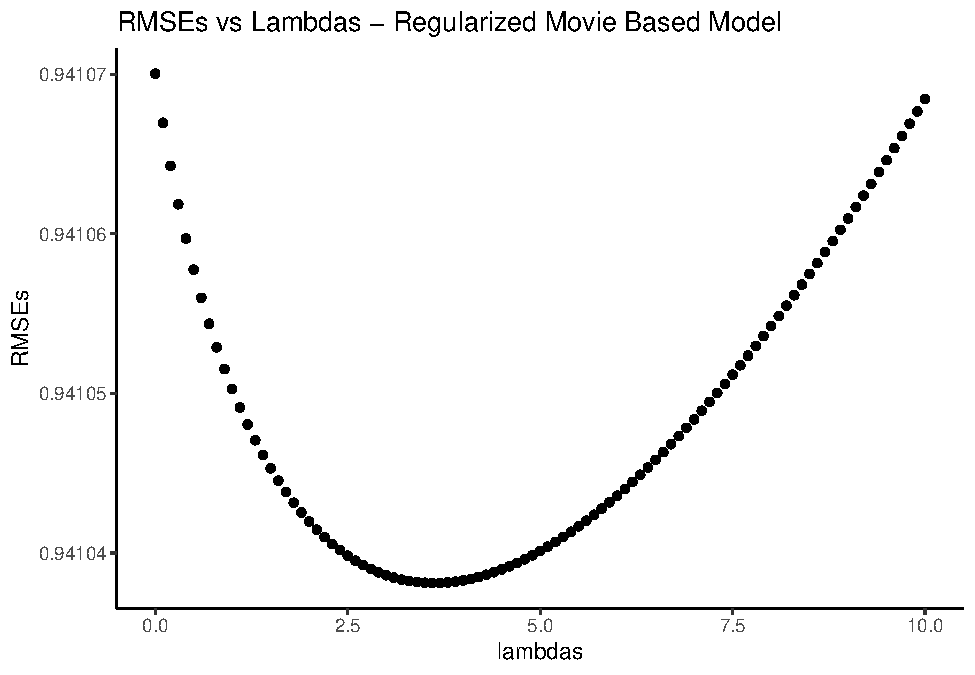
\includegraphics{MovieLens-Project-Code_files/figure-latex/unnamed-chunk-40-1} \end{center}

\begin{Shaded}
\begin{Highlighting}[]
\CommentTok{\# Get the lambda value that minimize the RMSE}
\NormalTok{min\_lambda }\OtherTok{\textless{}{-}}\NormalTok{ lambdas[}\FunctionTok{which.min}\NormalTok{(rmses)]}

\CommentTok{\# Predict the RMSE on the validation set}

\NormalTok{rmse\_regularized\_movie\_model }\OtherTok{\textless{}{-}} \FunctionTok{min}\NormalTok{(rmses)}

\CommentTok{\# Adding the results to the results dataset}

\NormalTok{results }\OtherTok{\textless{}{-}}\NormalTok{ results }\SpecialCharTok{\%\textgreater{}\%} \FunctionTok{add\_row}\NormalTok{(}\AttributeTok{model=}\StringTok{"Regularized Movie{-}Based Model"}\NormalTok{, }\AttributeTok{RMSE=}\NormalTok{rmse\_regularized\_movie\_model)}
\end{Highlighting}
\end{Shaded}

The RMSE on the \texttt{validation} dataset is \textbf{0.8635} and this
is very good. The Movie+User Based Model reaches the desidered
performance but applying the regularization techniques, can improve the
performance just a little.

\hypertarget{regularized-movieuser-model}{%
\subsubsection{Regularized Movie+User
Model}\label{regularized-movieuser-model}}

\begin{Shaded}
\begin{Highlighting}[]
\CommentTok{\# Calculate the average of all movies}

\NormalTok{mu\_hat }\OtherTok{\textless{}{-}} \FunctionTok{mean}\NormalTok{(edx}\SpecialCharTok{$}\NormalTok{rating)}

\CommentTok{\# Define a table of lambdas}

\NormalTok{lambdas }\OtherTok{\textless{}{-}} \FunctionTok{seq}\NormalTok{(}\DecValTok{0}\NormalTok{, }\DecValTok{15}\NormalTok{, }\FloatTok{0.1}\NormalTok{)}

\CommentTok{\# Compute the predicted ratings on validation dataset using different values of lambda}

\NormalTok{rmses }\OtherTok{\textless{}{-}} \FunctionTok{sapply}\NormalTok{(lambdas, }\ControlFlowTok{function}\NormalTok{(lambda) \{}

   \CommentTok{\# Calculate the average by user}
   
\NormalTok{   b\_i }\OtherTok{\textless{}{-}}\NormalTok{ edx }\SpecialCharTok{\%\textgreater{}\%}
      \FunctionTok{group\_by}\NormalTok{(movieId) }\SpecialCharTok{\%\textgreater{}\%}
      \FunctionTok{summarize}\NormalTok{(}\AttributeTok{b\_i =} \FunctionTok{sum}\NormalTok{(rating }\SpecialCharTok{{-}}\NormalTok{ mu\_hat) }\SpecialCharTok{/}\NormalTok{ (}\FunctionTok{n}\NormalTok{() }\SpecialCharTok{+}\NormalTok{ lambda))}
   
   \CommentTok{\# Calculate the average by user}
   
\NormalTok{   b\_u }\OtherTok{\textless{}{-}}\NormalTok{ edx }\SpecialCharTok{\%\textgreater{}\%}
      \FunctionTok{left\_join}\NormalTok{(b\_i, }\AttributeTok{by=}\StringTok{\textquotesingle{}movieId\textquotesingle{}}\NormalTok{) }\SpecialCharTok{\%\textgreater{}\%}
      \FunctionTok{group\_by}\NormalTok{(userId) }\SpecialCharTok{\%\textgreater{}\%}
      \FunctionTok{summarize}\NormalTok{(}\AttributeTok{b\_u =} \FunctionTok{sum}\NormalTok{(rating }\SpecialCharTok{{-}}\NormalTok{ b\_i }\SpecialCharTok{{-}}\NormalTok{ mu\_hat) }\SpecialCharTok{/}\NormalTok{ (}\FunctionTok{n}\NormalTok{() }\SpecialCharTok{+}\NormalTok{ lambda))}
   
   \CommentTok{\# Compute the predicted ratings on validation dataset}
   
\NormalTok{   predicted\_ratings }\OtherTok{\textless{}{-}}\NormalTok{ validation }\SpecialCharTok{\%\textgreater{}\%}
      \FunctionTok{left\_join}\NormalTok{(b\_i, }\AttributeTok{by=}\StringTok{\textquotesingle{}movieId\textquotesingle{}}\NormalTok{) }\SpecialCharTok{\%\textgreater{}\%}
      \FunctionTok{left\_join}\NormalTok{(b\_u, }\AttributeTok{by=}\StringTok{\textquotesingle{}userId\textquotesingle{}}\NormalTok{) }\SpecialCharTok{\%\textgreater{}\%}
      \FunctionTok{mutate}\NormalTok{(}\AttributeTok{pred =}\NormalTok{ mu\_hat }\SpecialCharTok{+}\NormalTok{ b\_i }\SpecialCharTok{+}\NormalTok{ b\_u) }\SpecialCharTok{\%\textgreater{}\%}
      \FunctionTok{pull}\NormalTok{(pred)}
   
   \CommentTok{\# Predict the RMSE on the validation set}
   
   \FunctionTok{return}\NormalTok{(}\FunctionTok{RMSE}\NormalTok{(validation}\SpecialCharTok{$}\NormalTok{rating, predicted\_ratings))}
\NormalTok{\})}

\CommentTok{\# plot the result of lambdas}

\NormalTok{df }\OtherTok{\textless{}{-}} \FunctionTok{data.frame}\NormalTok{(}\AttributeTok{RMSE =}\NormalTok{ rmses, }\AttributeTok{lambdas =}\NormalTok{ lambdas)}

\FunctionTok{ggplot}\NormalTok{(df, }\FunctionTok{aes}\NormalTok{(lambdas, rmses)) }\SpecialCharTok{+}
   \FunctionTok{theme\_classic}\NormalTok{()  }\SpecialCharTok{+}
   \FunctionTok{geom\_point}\NormalTok{() }\SpecialCharTok{+}
   \FunctionTok{labs}\NormalTok{(}\AttributeTok{title =} \StringTok{"RMSEs vs Lambdas {-} Regularized Movie+User Model"}\NormalTok{,}
        \AttributeTok{y =} \StringTok{"RMSEs"}\NormalTok{,}
        \AttributeTok{x =} \StringTok{"lambdas"}\NormalTok{)}
\end{Highlighting}
\end{Shaded}

\begin{center}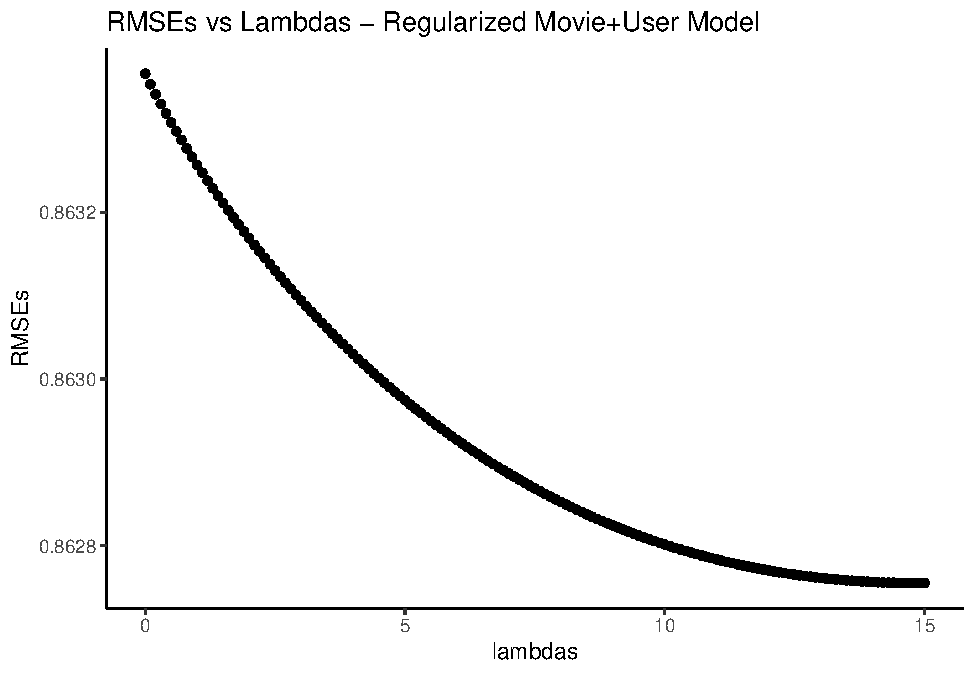
\includegraphics{MovieLens-Project-Code_files/figure-latex/unnamed-chunk-41-1} \end{center}

\begin{Shaded}
\begin{Highlighting}[]
\CommentTok{\# Get the lambda value that minimize the RMSE}

\NormalTok{min\_lambda }\OtherTok{\textless{}{-}}\NormalTok{ lambdas[}\FunctionTok{which.min}\NormalTok{(rmses)]}

\CommentTok{\# Predict the RMSE on the validation set}

\NormalTok{rmse\_regularized\_movie\_user\_model }\OtherTok{\textless{}{-}} \FunctionTok{min}\NormalTok{(rmses)}

\CommentTok{\# Adding the results to the results dataset}

\NormalTok{results }\OtherTok{\textless{}{-}}\NormalTok{ results }\SpecialCharTok{\%\textgreater{}\%} \FunctionTok{add\_row}\NormalTok{(}\AttributeTok{model=}\StringTok{"Regularized Movie+User Based Model"}\NormalTok{, }\AttributeTok{RMSE=}\NormalTok{rmse\_regularized\_movie\_user\_model)}
\end{Highlighting}
\end{Shaded}

The RMSE on the \texttt{validation} dataset is \textbf{0.8629}. The
Regularized Movie+User Based Model improves just a little the result of
the Non-Regularized Model.

\hypertarget{regularized-movieusergenre-model}{%
\subsubsection{Regularized Movie+User+Genre
Model}\label{regularized-movieusergenre-model}}

\begin{Shaded}
\begin{Highlighting}[]
\CommentTok{\# Calculate the average of all movies}

\NormalTok{mu\_hat }\OtherTok{\textless{}{-}} \FunctionTok{mean}\NormalTok{(edx}\SpecialCharTok{$}\NormalTok{rating)}

\CommentTok{\# Define a table of lambdas}

\NormalTok{lambdas }\OtherTok{\textless{}{-}} \FunctionTok{seq}\NormalTok{(}\DecValTok{0}\NormalTok{, }\DecValTok{15}\NormalTok{, }\FloatTok{0.1}\NormalTok{)}

\CommentTok{\# Compute the predicted ratings on validation dataset using different values of lambda}

\NormalTok{rmses }\OtherTok{\textless{}{-}} \FunctionTok{sapply}\NormalTok{(lambdas, }\ControlFlowTok{function}\NormalTok{(lambda) \{}

   \CommentTok{\# Calculate the average by user}
   
\NormalTok{   b\_i }\OtherTok{\textless{}{-}}\NormalTok{ edx }\SpecialCharTok{\%\textgreater{}\%}
      \FunctionTok{group\_by}\NormalTok{(movieId) }\SpecialCharTok{\%\textgreater{}\%}
      \FunctionTok{summarize}\NormalTok{(}\AttributeTok{b\_i =} \FunctionTok{sum}\NormalTok{(rating }\SpecialCharTok{{-}}\NormalTok{ mu\_hat) }\SpecialCharTok{/}\NormalTok{ (}\FunctionTok{n}\NormalTok{() }\SpecialCharTok{+}\NormalTok{ lambda))}
   
   \CommentTok{\# Calculate the average by user}
   
\NormalTok{   b\_u }\OtherTok{\textless{}{-}}\NormalTok{ edx }\SpecialCharTok{\%\textgreater{}\%}
      \FunctionTok{left\_join}\NormalTok{(b\_i, }\AttributeTok{by=}\StringTok{\textquotesingle{}movieId\textquotesingle{}}\NormalTok{) }\SpecialCharTok{\%\textgreater{}\%}
      \FunctionTok{group\_by}\NormalTok{(userId) }\SpecialCharTok{\%\textgreater{}\%}
      \FunctionTok{summarize}\NormalTok{(}\AttributeTok{b\_u =} \FunctionTok{sum}\NormalTok{(rating }\SpecialCharTok{{-}}\NormalTok{ b\_i }\SpecialCharTok{{-}}\NormalTok{ mu\_hat) }\SpecialCharTok{/}\NormalTok{ (}\FunctionTok{n}\NormalTok{() }\SpecialCharTok{+}\NormalTok{ lambda))}
   
\NormalTok{    b\_u\_g }\OtherTok{\textless{}{-}}\NormalTok{ edx }\SpecialCharTok{\%\textgreater{}\%}
      \FunctionTok{left\_join}\NormalTok{(b\_i, }\AttributeTok{by=}\StringTok{\textquotesingle{}movieId\textquotesingle{}}\NormalTok{) }\SpecialCharTok{\%\textgreater{}\%}
      \FunctionTok{left\_join}\NormalTok{(b\_u, }\AttributeTok{by=}\StringTok{\textquotesingle{}userId\textquotesingle{}}\NormalTok{) }\SpecialCharTok{\%\textgreater{}\%}
      \FunctionTok{group\_by}\NormalTok{(genre) }\SpecialCharTok{\%\textgreater{}\%}
      \FunctionTok{summarize}\NormalTok{(}\AttributeTok{b\_u\_g =} \FunctionTok{sum}\NormalTok{(rating }\SpecialCharTok{{-}}\NormalTok{ b\_i }\SpecialCharTok{{-}}\NormalTok{ mu\_hat }\SpecialCharTok{{-}}\NormalTok{ b\_u) }\SpecialCharTok{/}\NormalTok{ (}\FunctionTok{n}\NormalTok{() }\SpecialCharTok{+}\NormalTok{ lambda))}
   
   \CommentTok{\# Compute the predicted ratings on validation dataset}
   
\NormalTok{   predicted\_ratings }\OtherTok{\textless{}{-}}\NormalTok{ validation }\SpecialCharTok{\%\textgreater{}\%}
      \FunctionTok{left\_join}\NormalTok{(b\_i, }\AttributeTok{by=}\StringTok{\textquotesingle{}movieId\textquotesingle{}}\NormalTok{) }\SpecialCharTok{\%\textgreater{}\%}
      \FunctionTok{left\_join}\NormalTok{(b\_u, }\AttributeTok{by=}\StringTok{\textquotesingle{}userId\textquotesingle{}}\NormalTok{) }\SpecialCharTok{\%\textgreater{}\%}
      \FunctionTok{left\_join}\NormalTok{(b\_u\_g, }\AttributeTok{by=}\StringTok{\textquotesingle{}genre\textquotesingle{}}\NormalTok{) }\SpecialCharTok{\%\textgreater{}\%}
      \FunctionTok{mutate}\NormalTok{(}\AttributeTok{pred =}\NormalTok{ mu\_hat }\SpecialCharTok{+}\NormalTok{ b\_i }\SpecialCharTok{+}\NormalTok{ b\_u }\SpecialCharTok{+}\NormalTok{ b\_u\_g) }\SpecialCharTok{\%\textgreater{}\%}
      \FunctionTok{pull}\NormalTok{(pred)}
   
   \CommentTok{\# Predict the RMSE on the validation set}
   
   \FunctionTok{return}\NormalTok{(}\FunctionTok{RMSE}\NormalTok{(validation}\SpecialCharTok{$}\NormalTok{rating, predicted\_ratings))}
\NormalTok{\})}

\CommentTok{\# plot the result of lambdas}

\NormalTok{df }\OtherTok{\textless{}{-}} \FunctionTok{data.frame}\NormalTok{(}\AttributeTok{RMSE =}\NormalTok{ rmses, }\AttributeTok{lambdas =}\NormalTok{ lambdas)}

\FunctionTok{ggplot}\NormalTok{(df, }\FunctionTok{aes}\NormalTok{(lambdas, rmses)) }\SpecialCharTok{+}
   \FunctionTok{theme\_classic}\NormalTok{()  }\SpecialCharTok{+}
   \FunctionTok{geom\_point}\NormalTok{() }\SpecialCharTok{+}
   \FunctionTok{labs}\NormalTok{(}\AttributeTok{title =} \StringTok{"RMSEs vs Lambdas {-} Regularized Movie+User+Genre Model"}\NormalTok{,}
        \AttributeTok{y =} \StringTok{"RMSEs"}\NormalTok{,}
        \AttributeTok{x =} \StringTok{"lambdas"}\NormalTok{)}
\end{Highlighting}
\end{Shaded}

\begin{center}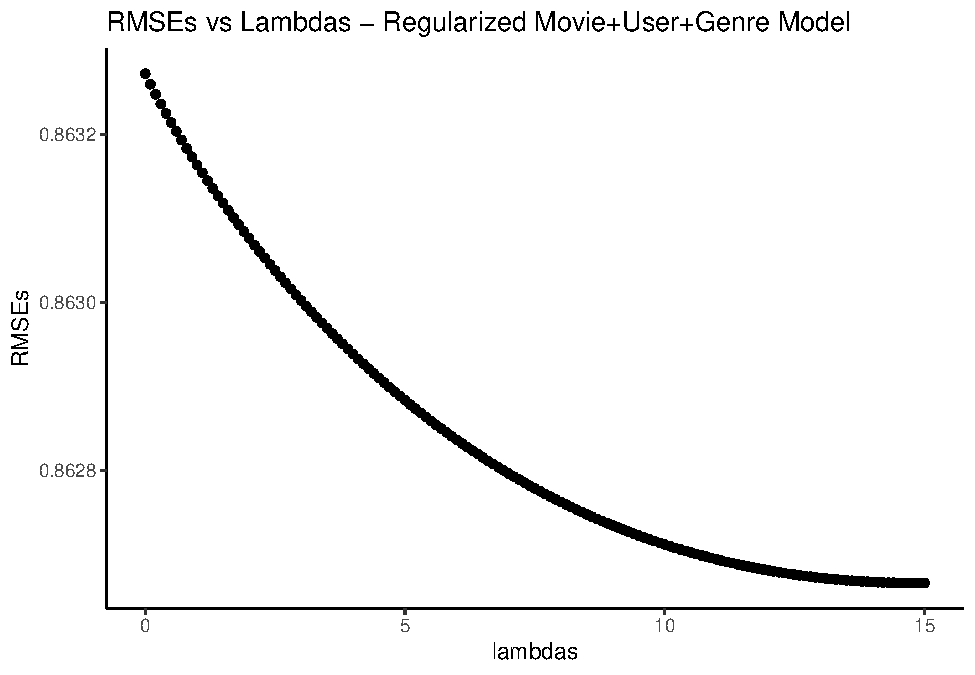
\includegraphics{MovieLens-Project-Code_files/figure-latex/unnamed-chunk-42-1} \end{center}

\begin{Shaded}
\begin{Highlighting}[]
\CommentTok{\# Get the lambda value that minimize the RMSE}

\NormalTok{min\_lambda }\OtherTok{\textless{}{-}}\NormalTok{ lambdas[}\FunctionTok{which.min}\NormalTok{(rmses)]}

\CommentTok{\# Predict the RMSE on the validation set}

\NormalTok{rmse\_regularized\_movie\_user\_genre\_model }\OtherTok{\textless{}{-}} \FunctionTok{min}\NormalTok{(rmses)}

\CommentTok{\# Adding the results to the results dataset}

\NormalTok{results }\OtherTok{\textless{}{-}}\NormalTok{ results }\SpecialCharTok{\%\textgreater{}\%} \FunctionTok{add\_row}\NormalTok{(}\AttributeTok{model=}\StringTok{"Regularized Movie+User+Genre Based Model"}\NormalTok{, }\AttributeTok{RMSE=}\NormalTok{rmse\_regularized\_movie\_user\_genre\_model)}
\end{Highlighting}
\end{Shaded}

The RMSE on the \texttt{validation} dataset is \textbf{0.8628} and this
is the best result of the builted models. The Regularized
Movie+User+Genre Based Model improves just a little the result of the
Non-Regularized Model. As the Non-Regularized Model, the \texttt{genre}
predictor doesn't improve significantly the model's performance.

\hypertarget{results}{%
\section{Results}\label{results}}

This is the summary results for all the model builted, trained on
\texttt{edx} dataset and validated on the \texttt{validation} dataset.

\begin{Shaded}
\begin{Highlighting}[]
\CommentTok{\# Shows the results}

\NormalTok{results }\SpecialCharTok{\%\textgreater{}\%} 
   \FunctionTok{kable}\NormalTok{() }\SpecialCharTok{\%\textgreater{}\%}
   \FunctionTok{kable\_styling}\NormalTok{(}\AttributeTok{bootstrap\_options =} \FunctionTok{c}\NormalTok{(}\StringTok{"striped"}\NormalTok{, }\StringTok{"hover"}\NormalTok{, }\StringTok{"condensed"}\NormalTok{, }\StringTok{"responsive"}\NormalTok{),}
             \AttributeTok{position =} \StringTok{"center"}\NormalTok{,}
             \AttributeTok{font\_size =} \DecValTok{10}\NormalTok{,}
             \AttributeTok{full\_width =} \ConstantTok{FALSE}\NormalTok{)}
\end{Highlighting}
\end{Shaded}

\begin{table}
\centering\begingroup\fontsize{10}{12}\selectfont

\begin{tabular}{l|r}
\hline
model & RMSE\\
\hline
Naive Mean-Baseline Model & 1.0525579\\
\hline
Movie-Based Model & 0.9410700\\
\hline
Movie+User Based Model & 0.8633660\\
\hline
Movie+User+Genre Based Model & 0.8632723\\
\hline
Regularized Movie-Based Model & 0.9410381\\
\hline
Regularized Movie+User Based Model & 0.8627554\\
\hline
Regularized Movie+User+Genre Based Model & 0.8626664\\
\hline
\end{tabular}
\endgroup{}
\end{table}

\hypertarget{conclusion}{%
\section{Conclusion}\label{conclusion}}

After training different models, it's very clear that \texttt{movieId}
and \texttt{userId} contribute more than the \texttt{genre} predictor.
Without regularization, the model can archieves and overtakes the
desidered peformance, but the best is the enemy of the good and applying
regularization and adding the \texttt{genre} predictor, it make possible
to reach a RSME of \textbf{0.8628} that is the best result for the
trained models.

\end{document}
